\documentclass[11pt,a4paper,twoside,english]{extarticle}
\usepackage[export]{adjustbox} % Nice alternative to minipage.
\usepackage{afterpage} % To give the title page its own geometry.
\usepackage[boxed,vlined,linesnumbered,resetcount,algosection]{algorithm2e} % For writing nice algorithms. 
\usepackage{amsmath} % Nice maths symbols.
\usepackage{amssymb} % Nice variable symbols.
\usepackage{amsthm} % Allows for nice definitions of theorem environments. 
\usepackage{array} % Allow for custom column widths in tables.
\usepackage{ltablex} % For long tables spanning multiple pages. % Must be before ARYDSHLN package!
\keepXColumns % Keeps the X column
\usepackage{arydshln} % Dashed lines using \hdashline \cdashline
%\usepackage[contents={}]{background} % Letting me add background overlays. 
\usepackage{bbm} % Gives Blackboard fonts. cf dsfont.
\usepackage{bm} % Bold math symbols.
\usepackage{calc} % Calculates widths of words. 
\usepackage{chngcntr} % Changing counters, e.g. with footnotes.
\usepackage{comment} % Allows large comment environments.
\usepackage{datetime} % For some  useful date time manipulation
\usepackage{datenumber}
\usepackage[final]{draftwatermark} % Gives a draft overlay. Use options [nostamp] or [final].
\usepackage{dsfont} % Nicer blackboard fonts. use \mathds{...}
\usepackage{emptypage} % Empty pages have no headers and footers.
\usepackage{enumitem} % Nice listing options in itemize and enumerate.
\usepackage{esdiff} % Gives nice differential operators.
\usepackage{esvect} % Gives nice vector arrows.
\usepackage{etoolbox}
\usepackage{fancyhdr} % Nice headers.
\usepackage{fancyvrb} % Better verbatim, and verb|| allowed in footnotes. 
\usepackage{listings} % The listings package for code. %% Needs to be loaded before float. 
\usepackage{float} % Nice figure placement.
\usepackage[T1]{fontenc} % Nice range of text characters and accents.
\usepackage[bottom]{footmisc} % Nice footnote formatting.
\usepackage{graphicx} % Include figures.
\usepackage[notquote]{hanging} % For indenting later lines in a paragraph. USE the 'noquote' option else the `'` is overwritten, and breaks in maths mode!
\usepackage{ifoddpage} % Checks for odd or even page.
\usepackage{imakeidx} % Makes the index.
\usepackage{indentfirst} % Indents the first paragraph.
\usepackage{letltxmacro} % For defining a nice SQRT symbol.
\usepackage[mathlines]{lineno} % For numbering lines.
\usepackage{lipsum} % Useful for adding jargon.
\usepackage{lmodern} % Load a font with all the characters
\usepackage{makecell} % Break table headers with multiline entries.
\usepackage{marginnote} % For nice margin notes.
\usepackage{mathtools} % Gives the colon equals symbol.
\usepackage[framed,numbered,autolinebreaks,useliterate]{mcode} % Inports Listings package ideal for MATLAB.
\usepackage[framemethod=tikz]{mdframed} % Gives nices boxed and sidesrules.
\usepackage{mleftright} % For better left and right delimiters.
\usepackage{multirow} % Nice table cells spanning many rows.
\usepackage{multicol} % If I want to use multiple columns.
\usepackage{nameref}
\usepackage[numbers, sort&compress]{natbib} % Nice references.
\usepackage{nicefrac} % Gives nice fractions for superscripts.
\usepackage{nomencl} % Gives a symbol nomenclature. 
\usepackage[super]{nth} % Gives nice ordinal superscripts, eg 1st, 2nd, etc.
\usepackage{pifont} % For the check and cross marks
\usepackage{physics} % Nice partial derivatives and BRAKET notation.
\usepackage{ragged2e} % For nice allignment.
%\usepackage[norefs]{refcheck} % Can show any unused references.
\usepackage{romannum} % Nice typing for roman numerals.
\usepackage{rotating} % For sideways figures.
\usepackage[scr,scaled=1.1]{rsfso} % Gives Script fonts which are not so slanted. 
\usepackage{scalerel} % Allows the scaling of symbols. 
\usepackage{setspace} % Ideal for increasing line spacing. E.g.  \doublespacing
\usepackage[binary-units=true]{siunitx} % Nice formating of units.
\usepackage{sidenotes} % Nice margin figures and margin tables. 
\usepackage{subcaption} % Side by side figures.
\usepackage{thmtools}
\usepackage{tikz} % Nice diagrams.
\usepackage{titling} % Gives a bit of extra control around maketitle. 
\usepackage{tocbasic} % For better TOC alignment
\usepackage[nottoc]{tocbibind} % Gives nices Table of Contents
\usepackage[textsize=footnotesize]{todonotes} % A nice TODO list. [disable] to supress.
\usepackage{transparent} % Allows for transparent text. 
\usepackage[normalem]{ulem} % For striked through text.
\usepackage[hyphens]{url} % Allows urls to break on hyphens
\usepackage{usebib} % For citing a paper's title.
%\usepackage[table]{xcolor} % This is useful for making greyed table cells, nice for headers. Known preamble placement issues.
\usepackage{wasysym} % Gives some nice misc symbols, such as markers.
\usepackage{wrapfig}
\usepackage{xifthen}% Provides \isempty test.
\usepackage{xparse} % Gives \NewDocumentEnvironment which has nice optional argument handling.
\usepackage{xspace} % Gives nice spacing for commands.
%%%% Generally HYPERREF should be imported last. %%%%
\usepackage[colorlinks=true,linkcolor=black,urlcolor=black,citecolor=black,anchorcolor=black,breaklinks]{hyperref} % Colour links.
%%%% Should be loaded after hyperref. %%%%
\usepackage{cleveref} % Gives smart referencing. %% After Hyperref
\usepackage[margin=10pt,font=small,labelfont=bf,labelsep=endash,figurewithin=section,tablewithin=section]{caption} % Caption figures and tables nicely. %% After cleveref.
\usepackage[top=20mm,bottom=20mm,left=20mm, right=30mm, heightrounded, marginparwidth=24mm,  marginparsep=3mm, headsep=10mm]{geometry} % Use nice margins. Does give a small change in the default page margins. 
%[left=60mm,right=26mm,top=30mm,bottom=29mm, heightrounded, marginparwidth=41mm, marginparsep=8mm, headsep=10mm]


% Getting SI options setup.
\sisetup{range-phrase=--, range-units=single}


% Ensures subsubsections are numbered.
\setcounter{secnumdepth}{3}

% Makes math bold in headers and titles. 
\makeatletter
\g@addto@macro\bfseries{\boldmath}
\makeatother

\makeindex

\makenomenclature
% The column width for any nomenclature. 
\setlength\nomlabelwidth{0.2\linewidth}


% Set the table of content depth to only subsections. 
\setcounter{tocdepth}{2}


%\hbadness=10000 % Supresses bad box warnings


% Present the references in the order they are used.
%\bibliographystyle{unsrtnat} % Sorted by order of use.
%\bibliographystyle{plainnat} % Alphabetical. 
\bibliographystyle{customplainnat} % Alphabetical, with a more uniform formatting.
% Reduce spacing between references. 
\setlength{\bibsep}{0pt plus 0.3ex}
% For the usebib package to find the references. 
\bibinput{references}


% Listing -> Code in environment labels.
\renewcommand{\lstlistingname}{Code}
\renewcommand{\lstlistlistingname}{List of codes}
\crefname{listing}{code}{code}  
\Crefname{listing}{Code}{Codes}
\AtBeginDocument{\counterwithin{lstlisting}{section}} % Ensures these are numbered enough
\newfloat{lstfloat}{htbp}{lop} % environment for placing lisings in to make them float. 
% Make list of listings/code have the same inter-chapter spacing as other lists.
\let\Chapter\chapter
\def\chapter{\addtocontents{lol}{\protect\addvspace{10pt}}\Chapter}
\makeatletter
\patchcmd{\@chapter}{\chaptermark{#1}}{%
    \chaptermark{#1}%
    \addtocontents{lol}{\protect\addvspace{10\p@}}%
}{\typeout{Chapters patched for list-of-listings.}}{\typeout{Could not patch chapters for list-of-listings.}}
\makeatother

% List of Algorithms (NB, requires french spelling of 'algorithmes')
\renewcommand*{\listalgorithmcfname}{List of algorithms}
\newcommand{\listofalgorithmes}{\tocfile{\listalgorithmcfname}{loa}}



% Have theorems and lemmas be referenced by name if applicable.
\makeatletter
\renewrobustcmd{\cref}{\@osmcref{cref}}
\renewrobustcmd{\Cref}{\@osmcref{Cref}}
\def\@osmcref#1#2{%
    \begingroup
    \ifcsundef{r@#2}
    {}
    {\expandafter\expandafter\expandafter\expandafter\expandafter
        \expandafter\expandafter\def
        \expandafter\expandafter\expandafter\expandafter\expandafter
        \expandafter\expandafter\@osmcref@name
        \expandafter\expandafter\expandafter\expandafter\expandafter
        \expandafter\expandafter{%
            \expandafter\expandafter\expandafter
            \@thirdoffive\csname r@#2\endcsname}}%
    \ifcsundef{r@#2@cref}
    {}
    {\cref@gettype{#2}{\@osmcref@type}}%
    \ifboolexpr{not test {\ifdefvoid{\@osmcref@name}}
        and (test {\ifdefstring{\@osmcref@type}{theorem}}
        or test {\ifdefstring{\@osmcref@type}{lemma}}
        or test {\ifdefstring{\@osmcref@type}{corollary}})}
    {\nameref{#2} (\@cref{#1}{#2})}
    {\@cref{#1}{#2}}%
    \endgroup
}
\makeatother
% Give bold names to definitions and similar environments. 
\makeatletter
\def\th@plain{%
    \thm@notefont{}% same as heading font
    \itshape % body font
}
\def\th@definition{%
    \thm@notefont{}% same as heading font
    \normalfont % body font
}
\makeatother
% Giving correct theorem and lemma environments. 
\newtheorem{theorem}{Theorem}[section]
\newtheorem{corollary}{Corollary}[theorem]
\newtheorem{proposition}[theorem]{Proposition}
\newtheorem{lemma}[theorem]{Lemma}
\theoremstyle{definition}
\newtheorem{remark}{Remark}[theorem]
\newtheorem{definition}{Definition}[section]
\newtheorem{assumption}{Assumption}[section]
\newtheorem{proofof}{Proof}[theorem]
\AtEndEnvironment{proofof}{\qed}
% Naming these nicely.
\crefname{lemma}{lemma}{lemmas}
\Crefname{lemma}{Lemma}{Lemmas}
\crefname{theorem}{theorem}{theorems}
\Crefname{theorem}{Theorem}{Theorems}
\crefname{corollary}{corollary}{corollaries}
\Crefname{corollary}{Corollary}{Corollaries}
\Crefname{proposition}{proposition}{propositions}
\Crefname{proposition}{Proposition}{Propositions}
\crefname{remark}{remark}{remarks}
\Crefname{remark}{Remark}{Remarks}
\crefname{definition}{definition}{definitions}
\Crefname{definition}{Definition}{Definitions}
\crefname{assumption}{assumption}{assumptions}
\Crefname{assumption}{Assumption}{Assumptions}
% Change the end of proof symbol
\renewcommand\qedsymbol{\textbf{QED}}
% Making the proof in bold so it stands out more. 
\let\oldproofname=\proofname
\renewcommand{\proofname}{\rm\bf{\oldproofname}}

% Give bold names to definitions and similar environments. 
\makeatletter
\def\th@plain{%
    \thm@notefont{}% same as heading font
    \itshape % body font
}
\def\th@definition{%
    \thm@notefont{}% same as heading font
    \normalfont % body font
}
\makeatother

% Nice paragraph indents.
\setlength{\parindent}{5em}
\setlength{\parskip}{0.5\baselineskip}

% Giving the references the right title.
\renewcommand{\bibname}{References}
\renewcommand{\listfigurename}{List of figures}
\renewcommand{\listtablename}{List of tables}


% Removes hyphenation
\tolerance=1
\emergencystretch=\maxdimen
\hyphenpenalty=10000
\hbadness=10000

% To change the spacing in lists
%\setlist{noitemsep} % or \setlist{noitemsep} to leave space around whole list
%\setenumerate{itemsep=-0.4em,topsep=0.5em} % Seems to look nice.

% Custom column widths using C{2cm}, L, R, etc.
\newcolumntype{L}[1]{>{\raggedright\let\newline\\\arraybackslash\hspace{0pt}}m{#1}}
\newcolumntype{C}[1]{>{\centering\let\newline\\\arraybackslash\hspace{0pt}}m{#1}}
\newcolumntype{R}[1]{>{\raggedleft\let\newline\\\arraybackslash\hspace{0pt}}m{#1}}

% Gives a nice column separation in multicolumn mode.
\setlength{\columnsep}{5mm}

% Figure environment for use in multicolumn. To put in captions use \captionof{figure}{content of caption}.
\newenvironment{Figure}
{\par\medskip\noindent\minipage{\linewidth}}
{\endminipage\par\medskip}

% Gives the nice SQRT symbol.
\makeatletter
\let\oldr@@t\r@@t
\def\r@@t#1#2{%
	\setbox0=\hbox{$\oldr@@t#1{#2\,}$}\dimen0=\ht0
	\advance\dimen0-0.2\ht0
	\setbox2=\hbox{\vrule height\ht0 depth -\dimen0}%
	{\box0\lower0.4pt\box2}}
\LetLtxMacro{\oldsqrt}{\sqrt}
\renewcommand*{\sqrt}[2][\ ]{\oldsqrt[#1]{#2}}
\makeatother

\DeclareMathOperator{\sign}{sign}
\DeclareMathOperator*{\argmin}{argmin}
\DeclareMathOperator*{\argmax}{argmax}
\newcommand{\indicatorfn}{\mathds{1}}
\newcommand{\iconst}{\mathrm{i}}
\newcommand{\econst}{\mathrm{e}}
\newcommand{\erfinv}{\mathrm{inverf}}
\newcommand{\inverf}{\erfinv}

% A nice conditional expectation environment for use with probability spaces. 
% Based on Physics package. 
% \conExp[Measure][Subset]{Argument}{Condition}   (Condition is optional field)
\DeclareDocumentCommand\conExp{s o o m g}{
    % s : star, to use non scaling parenthesese.
    % o : optional, probability measure.
    % o : optional, set over which expectation is taken.
    % m : mandatory, argument.
    % g : optional, condition.
    \IfBooleanTF{#1}{}{\trigbraces}{\mathbb{E}\IfNoValueTF{#2}{}{^{#2}}\IfNoValueTF{#3}{}{_{#3}}}(#4\IfNoValueTF{#5}{}{\IfBooleanTF{#1}{\mid}{\,\middle|\,}#5})
}

\DeclareDocumentCommand\conVar{s o o m g}{
    % s : star, to use non scaling parenthesese.
    % o : optional, probability measure.
    % o : optional, set over which expectation is taken.
    % m : mandatory, argument.
    % g : optional, condition.
    \IfBooleanTF{#1}{}{\trigbraces}{\mathbb{V}\IfNoValueTF{#2}{}{^{#2}}\IfNoValueTF{#3}{}{_{#3}}}(#4\IfNoValueTF{#5}{}{\IfBooleanTF{#1}{\mid}{\,\middle|\,}#5})
}

\DeclareDocumentCommand\quadVar{s m g g}{
    % s : star, to use non scaling parenthesese.
    % m : mandatory, first argument.
    % g : optional, evaluation time.
    % g : optional, second argument.
    \IfBooleanTF{#1}{\expval*{#2\IfNoValueF{#4}{,#4}}\IfNoValueF{#3}{_{#3}}}{\expval{#2\IfNoValueF{#4}{,#4}}\IfNoValueF{#3}{_{#3}}}
}

\newlength{\LowercaseLength}
\AtBeginDocument{\settoheight{\LowercaseLength}{a}} % after \normalsize
\DeclareDocumentCommand\lorder{s m}{%
    \IfBooleanTF{#1}{}{\trigbraces}{\resizebox{!}{\LowercaseLength}{$\mathcal{O}$}}(#2)%
}


% Number equations down to the subection level, e.g. 1.2.3 is the third equation in
% subsection 2 of section 1.
\numberwithin{equation}{section}
\newcommand*\tageq{\refstepcounter{equation}\tag{\theequation}}
% Ensure equations are correctly formatted with cleverref
\crefname{equation}{}{}
\creflabelformat{equation}{(#2#1#3)}


% This makes the footnote counter reset in each section.
\counterwithin*{footnote}{section}

% Nice spacing in the first fow of a table
\newcommand{\firstrowspacing}{\rule{0pt}{2.6ex}}
% For a more open look in tables.
\setlength\extrarowheight{3pt} 

% Some corporate names we may need to append a \textsuperscript{\textregistered} into. 
\newcommand{\nag}{NAG\xspace}
\newcommand{\arm}{Arm\xspace}
\newcommand{\intel}{Intel\xspace}
\newcommand{\openmp}{OpenMP\xspace}
\newcommand{\amd}{AMD\xspace}
\newcommand{\ibm}{IBM\xspace}
\newcommand{\nvidia}{Nvidia\xspace}
\newcommand{\icdf}{inverse cumulative density function\xspace}
\newcommand{\rng}{random number generator\xspace}
\newcommand{\PhiInverse}{$ \Phi^{-1}(\cdot) $\xspace}
\newcommand{\Ito}{It\^{o}\xspace}
\newcommand{\BDG}{Burkholder-Davis-Gundy\xspace}
\newcommand{\CIR}{Cox-Ingersoll-Ross\xspace}


% The nice headers and footers.
\pagestyle{fancy}
% Modifying the header and footer styles for chapters and sections. 
\renewcommand{\sectionmark}[1]{\markboth{#1}{#1}}

% Specifying the headers and footers. 
\fancyhf{}
\renewcommand*{\headrulewidth}{1pt}%
\fancyhead[LO]{\nouppercase{\leftmark}}
\fancyhead[RE]{\nouppercase{\rightmark}}
\fancyhead[LE,RO]{\thepage}
\fancypagestyle{plain}{%
	\fancyhf{}%
	\renewcommand*{\headrulewidth}{0pt}%
}
\cfoot{}%\thepage}





% Make margin notes small
\renewcommand*{\marginfont}{\noindent \footnotesize}
%\reversemarginpar % If I want a thick margin by the binding.
\renewcommand\raggedrightmarginnote{\sloppy}
\renewcommand\raggedleftmarginnote{\sloppy}


% Gives a nice quote environment.
\NewDocumentEnvironment{myquote}{O{}}{%
	\begin{center}
		\begin{minipage}{0.85\linewidth}
			\vspace{1ex}
			\centering \itshape \justifying}
		{%
			\ifthenelse{\isempty{#1}}{}{
			\begin{flushright}%The author/source.
				\normalfont #1
			\end{flushright}}
						\vspace{1ex}
		\end{minipage}
	\end{center}
}

% Gives a nice siderule environment. e.g. \begin{siderules}
\newmdenv[topline=false,bottomline=false,rightline=false,skipabove=\topsep,skipbelow=\topsep,backgroundcolor=none]{siderules}

% For a numbered and description. Use inside enumerate, \litem{Something} etc. 
\newcommand\litem[1]{\item{\textit{#1} \\ \hfill \vspace*{-1.5ex} \\ \indent}}

% Nice spacing in lists
%\setlist{listparindent=\parindent,parsep=1ex} 

% This alligns figures in the adjust box environment to the inner margin. 
\newcommand{\aligninner}{\ifoddpage \raggedright \else \raggedleft \fi}%


% Gives a nice aligned figure environment, where figures are flush to the inner margin overflowing off the outer margin first. Useful for very wide figures, or set of lots of fub figures. 
\NewDocumentEnvironment{myalignedfigure}{O{1.3} O{htb}}{% fractional_linewidth,  position
	\begin{figure}[#2]
	\checkoddpage
	\edef\whichside{\ifoddpage left\else right\fi}
		\begin{adjustbox}{\whichside, minipage=#1\linewidth}}
		{%
		\end{adjustbox}
	\end{figure}
	}

% Gives a nice draft text.
\SetWatermarkScale{1}
\SetWatermarkLightness{0.9}

% The oxford comma from cref for multiple citations. 
\newcommand{\creflastconjunction}{, and\nobreakspace}

% Allows for bold face typed text fonts for computer modern font family. Useful in listings. 
\DeclareFontShape{OT1}{cmtt}{bx}{n}{<5><6><7><8><9><10><10.95><12><14.4><17.28><20.74><24.88>cmttb10}{}



% Allowing alignat to have repeating alignment options. 
\makeatletter
\def\align@preamble@r{%
    \hfil
    \strut@
    \setboxz@h{\@lign$\m@th\displaystyle{##}$}%
    \ifmeasuring@\savefieldlength@\fi
    \set@field
    \tabskip\z@skip}
\def\align@preamble@l{%
    \strut@
    \setboxz@h{\@lign$\m@th\displaystyle{{}##}$}%
    \ifmeasuring@\savefieldlength@\fi
    \set@field
    \hfil
    \tabskip\alignsep@}
\def\align@preamble@c{%
    \hfil
    \strut@
    \setboxz@h{\@lign$\m@th\displaystyle{{}##}$}%
    \ifmeasuring@\savefieldlength@\fi
    \set@field
    \hfil
    \tabskip\alignsep@
}
\def\setalignpreamble#1{\def\align@preamble{}\x@setalignpreamble#1\relax}
\def\x@setalignpreamble#1{%
    \ifx\relax#1\else
    \edef\align@preamble{%
        \expandafter\unexpanded\expandafter{\align@preamble}%
        &\span\expandafter\noexpand\csname align@preamble@#1\endcsname}%
    \expandafter\x@setalignpreamble
    \fi}


% A more extreme version of shortintertext
\newcommand\prefixtext[1]{%
    \ifvmode\else\\\@empty\fi
    \noalign{%
        \penalty0%
        \vbox{\mathstrut}%
        \penalty10000%
        \vskip-\baselineskip
        \penalty10000%
        \vbox to 0pt{%
            \normalbaselines
            \ifdim\linewidth=\columnwidth
            \else
            \parshape\@ne
            \@totalleftmargin\linewidth
            \fi
            \vss
            \noindent#1\par}%
        \penalty10000%
        \vskip-\baselineskip}%
    \penalty10000}


% Gives a nice thousand separator. 
\sisetup{group-separator = \text{\,}, group-minimum-digits=5}

% Makes thead the normal font size. 
\renewcommand\theadfont{}

% \fp[precision]{Argument} (Condition is optional field)
\DeclareDocumentCommand\fp{o m}{
    % s : star, to use non scaling parenthesese.
    % o : optional, precision level.
    % m : mandatory, argument.
    \bar{#2}\IfNoValueTF{#1}{}{^{(#1)}}
}
% \fpSQRT[precision]{Argument} 
\DeclareDocumentCommand\fpSQRT{s o m}{
    % s : star, to use non scaling parenthesese.
    % o : optional, precision level.
    % m : mandatory, argument.
    \mathinner{\IfBooleanTF{#1}{}{\trigbraces}{\overline{\mathrm{sqrt}}\IfNoValueTF{#2}{}{^{(#2)}}}(#3)}
}
\DeclareDocumentCommand\fpRound{s o m}{
    % s : star, to use non scaling parenthesese.
    % o : optional, precision level.
    % m : mandatory, argument.
    \mathinner{\IfBooleanTF{#1}{}{\trigbraces}{\mathscr{R}}(#3\IfNoValueTF{#2}{}{;{#2}})}
}
\DeclareDocumentCommand\support{s m}{
    % s : star, to use non scaling parenthesese.
    % m : mandatory, argument.
    \mathinner{\IfBooleanTF{#1}{}{\trigbraces}{\mathrm{supp}}(#2)}
}

% Making some circled operators. (use \ocircle for a smaller circle)
\makeatletter
\newcommand\incircbin
{%
  \mathpalette\@incircbin
}
\newcommand\@incircbin[2]
{%
  \mathbin%
  {%
    \ooalign{\hidewidth$#1#2$\hidewidth\crcr$#1\bigcirc$}%
  }%
}
\newcommand{\fpPlus}{\incircbin{+}}
\newcommand{\fpMinus}{\incircbin{-}}
\newcommand{\fpTimes}{\incircbin{\times}}
\newcommand{\fpDivide}{\incircbin{\divisionsymbol}}
\newcommand{\fpOp}{\incircbin{\ast}}
\makeatother

%\newcommand{\fpPlus}{\oplus}
%\newcommand{\fpMinus}{\ominus}
%\newcommand{\fpTimes}{\otimes}
%\newcommand{\fpDivide}{\oslash} 
%\newcommand{\fpOp}{\circledast}


%\newcommand{\sumfine}{\mathop{{{\sum}^{\mathrlap{\,\mathrm{f}}}}}}
%\newcommand{\sumcoarse}{\mathop{{{\sum}^{\mathrlap{\,\mathrm{c}}}}}}
\DeclareDocumentCommand\sumfine{g g}{
    % g : optional, subscript.
    % g : optional, superscript.
    \mathop{{{\sum}_{\mathrlap{\mathrm{f}}}}}\limits\IfNoValueF{#1}{_{#1}}\IfNoValueF{#2}{^{#2}}\,
}
\DeclareDocumentCommand\sumcoarse{g g}{
    % g : optional, subscript.
    % g : optional, superscript.
    \mathop{{{\sum}_{\mathrlap{\mathrm{c}}}}}\limits\IfNoValueF{#1}{_{#1}}\IfNoValueF{#2}{^{#2}}\,
}

\DeclareDocumentCommand\supfine{g}{
    % g : optional, subscript.
    \mathop{\mathrm{sup}^{\mathrlap{\mathrm{f}}}}\IfNoValueF{#1}{_{#1}}\,
}
\DeclareDocumentCommand\supcoarse{g}{
    % g : optional, subscript.
    \mathop{\mathrm{sup}^{\mathrlap{\mathrm{c}}}}\IfNoValueF{#1}{_{#1}}\,
}



% For usage in align environments. 
\newcommand\phantomrel[1]{\mathrel{\phantom{#1}}}
\newcommand\phantombin[1]{\mathbin{\phantom{#1}}}

% For defining some paired delimited items, such as set, floor, ceil, etc, where the spacing is correct and scaling is supressed with a * notation, e.g. \set{} and \set*{}
\NewDocumentCommand\xDeclarePairedDelimiter{mmm}
{%
    \NewDocumentCommand#1{som}{%
        \IfNoValueTF{##2}
        {\IfBooleanTF{##1}{#2##3#3}{\mleft#2##3\mright#3}}
        {\mathopen{##2#2}##3\mathclose{##2#3}}%
    }%
}
\xDeclarePairedDelimiter{\set}{\lbrace}{\rbrace}
\xDeclarePairedDelimiter{\floor}{\lfloor}{\rfloor}
\xDeclarePairedDelimiter{\ceil}{\lceil}{\rceil}
\xDeclarePairedDelimiter{\parens}{(}{)} 

\DeclareDocumentCommand\logtwo{}{\trigbraces{{\logarithm}_{2}}}
\DeclareDocumentCommand\logten{}{\trigbraces{{\logarithm}_{10}}}

% Allowing verbatim in footnotes. 
\VerbatimFootnotes

\newcommand{\cmark}{\ding{51}}%
\newcommand{\xmark}{\ding{55}}%

% Making a 4-way difference operator (looks like the D'Alembertian)
\makeatletter
\newcommand{\fourdiff}{{\mathpalette\fourdiff@\relax}}%{\mathop{\mathpalette\fourdiff@\relax}}
\newcommand{\fourdiff@}[2]{%
  \begingroup
  \sbox\z@{$\m@th#1\square$}%
  \dimen0=\fontdimen8
    \ifx#1\displaystyle\textfont\else
    \ifx#1\textstyle\textfont\else
    \ifx#1\scriptstyle\scriptfont\else
    \scriptscriptfont\fi\fi\fi3
  \makebox[\wd\z@]{%
    \hbox to \ht\z@{%
      \vrule width \dimen0
      \kern-\dimen0
      \vbox to \ht\z@{
        \hrule height \dimen0 width \ht\z@
        \vss
        \hrule height 2\dimen0
      }%
      \kern-2.5\dimen0
      \vrule width 2.5\dimen0
    }%
  }%
  \endgroup
}
\makeatother



\newcommand{\contradiction}{\scaleobj{1.5}{\text{\textreferencemark}}}


% So Roman page numbers are right aligned. and proper spacing between section numbers and captions
\DeclareTOCStyleEntry[numwidth=3.5em]{tocline}{figure}% for figure entries
\DeclareTOCStyleEntries[
  level:=figure,
  indent:=figure,
  numwidth:=figure,
  dynnumwidth% enlarges numwidth automatically if the entry number is too long; needs an additional run
]{tocline}{table,lstlisting,algocf,todo}
\DeclareTOCStyleEntries[
  rightindent=10em,
  pagenumberbox=\pagenumberbox
]{tocline}{section,subsection,subsubsection,paragraph,subparagraph,figure,table,lstlisting,algocf,todo}
\newcommand*\pagenumberbox[1]{\mbox{\hspace{0em}#1}}



%%%% Patching some math environments from AMS for better line numbering. %%%%

%% Patch 'normal' math environment: (currently unused, but good to have)
% \newcommand*\linenomathpatch[1]{%
%   \expandafter\pretocmd\csname #1\endcsname {\linenomath}{}{}%
%   \expandafter\pretocmd\csname #1*\endcsname{\linenomath}{}{}%
%   \expandafter\apptocmd\csname end#1\endcsname {\endlinenomath}{}{}%
%   \expandafter\apptocmd\csname end#1*\endcsname{\endlinenomath}{}{}%
% }
%% Patch AMS math environment:
\newcommand*\linenomathpatchAMS[1]{%
    \expandafter\pretocmd\csname #1\endcsname {\linenomathAMS}{}{}%
    \expandafter\pretocmd\csname #1*\endcsname{\linenomathAMS}{}{}%
    \expandafter\apptocmd\csname end#1\endcsname {\endlinenomath}{}{}%
    \expandafter\apptocmd\csname end#1*\endcsname{\endlinenomath}{}{}%
}

%% Definition of \linenomathAMS depends on whether the mathlines option is provided
\expandafter\ifx\linenomath\linenomathWithnumbers
\let\linenomathAMS\linenomathWithnumbers
%% The following line gets rid of an extra line numbers at the bottom:
\patchcmd\linenomathAMS{\advance\postdisplaypenalty\linenopenalty}{}{}{}
\else
\let\linenomathAMS\linenomathNonumbers
\fi

% \linenomathpatch{equation} %% <- unnecessary, equation is already patched
\linenomathpatchAMS{gather}
\linenomathpatchAMS{multline}
\linenomathpatchAMS{align}
\linenomathpatchAMS{alignat}
\linenomathpatchAMS{flalign}

% Mark the style as style=C and it will highlight more keywords. 
\lstdefinestyle{C}{
    language=C,
    morekeywords={omp,simd,reduction,simdlen,declare,inline,bool,restrict,half},
    otherkeywords={\#pragma,\_\_fp16,\#if,\#elif,\#else,\#endif,\#ifdef}
}

% Making an independent symbol.
\newcommand\independent{\protect\mathpalette{\protect\independenT}{\perp}}
\def\independenT#1#2{\mathrel{\rlap{$#1#2$}\mkern2mu{#1#2}}}

% Increase algorithm spacing between box and caption and font size.
\SetAlCapSkip{1em}
\SetAlCapNameFnt{\small}
\SetAlCapFnt{\small}


\newcommand{\singlecodeline}[1]{\\[1em]\centerline{\lstinline[basicstyle=\ttfamily]$#1$}\\[1em]}


\title{\bfseries Getting started with approximate random variables:\\[0.5em] a brief guide for practitioners}
\author{\href{mailto:oliver.sheridan-methven@hotmail.co.uk}{Oliver Sheridan-Methven}%
\thanks{\href{mailto:oliver.sheridan-methven@hotmail.co.uk}%
{\texttt{oliver.sheridan-methven@hotmail.co.uk}}}
}
\date{Version 0.1\\[1em]
Last updated \datedayname\ \nth{\number\day} \monthname\  \number\year}

% Allowing use to make some highlighted entries in Verbatim. 
\newcommand\highlightverb[1]{\underline{\textbf{#1}}}


\begin{document}
%\linenumbers
\pagestyle{empty}
\maketitle
\pagenumbering{arabic}

\begin{abstract}
We introduce the idea of \emph{approximate random variables} and discuss when they are useful. We provide code bundles in Python and C which demonstrate various implementations and use-cases, showing key results, and how to obtain these yourself using the code provided.  
\end{abstract}


\vfill
\centerline{\includegraphics[width=\linewidth]{accuracy_and_precision}}
\vfill

\clearpage
\tableofcontents
\cleardoublepage
\pagenumbering{arabic}
\pagestyle{fancy}

\clearpage
\section{Prerequisites for the demonstrations}

The demonstrations we provide will mostly be written in Python, and a few higher performance versions will be in C. For the Python code, we will be using Python~3, although it should all be easily portable to Python~2 with minimal modification. The Python files can either be run from a Python IDLE, or from the command line, whichever is easier. We assume a Unix or GNU/Linux based operating system. The C files will come with their own makefiles\footnote{We actually provide these as ``\verb|.sh|'' files, which can be readily adapted or copied directly to the terminal.}, and will usually assume access to the \texttt{gcc} compiler. Some of the C programs are not hardware agnostic, and will require altering the makefiles in places. For some applications, we may be comparing performance against \intel or \nag libraries, and assessing performance on \intel, \arm, or even \nvidia hardware. As a minimum, we will require the user has 
\begin{itemize}
\item The GNU scientific library (GLS) and the \texttt{gcc} compiler.
\end{itemize}
Further to this, some of the more advanced demonstrations may require any of the following:
\begin{itemize}
\item The \intel maths kernel library (MKL), the vector statistics library (VSL), and the \texttt{icc} compiler. 
\item The \nag library. 
\item The \arm \texttt{armclang} compiler.
\item The \nvidia \texttt{nvcc} compiler.
\end{itemize} 
Similarly, we will assume access to appropriate hardware from either \intel, \arm, or \nvidia where appropriate. We assume when compiling that the user has also setup the default paths to find the required header files and libraries by appropriately setting the environment variables \verb|LIBRARY_PATH|, \verb|LD_LIBRARY_PATH|, and \verb|C_INCLUDE_PATH|.

We will try an keep the Python packages used to a minimum, although some of the notable packages which are used within our code include: \texttt{numpy}, \texttt{pandas}, \texttt{scipy}, \texttt{matplotlib}, \texttt{progressbar2}, \texttt{bisect}, \texttt{timeit}, etc. 

To give an idea of the more relevant files contained, the user should expect a file structure similar to:
\begin{lstfloat}[H]
\begin{Verbatim}[commandchars=\\\{\}]
approximate_random_variables/
|-- ... \highlightverb{The files to read} ...
|-- approximate_random_variables.pdf
|-- ... \highlightverb{The Python approximations}  ...
|-- approximate_gaussian_distribution.py
|-- approximate_gaussian_distribution_demonstrations.py
|-- approximate_non_central_chi_squared.py
|-- approximate_non_central_chi_squared_demonstrations.py
|-- ... \highlightverb{The C/C++ approximations} ...
|-- piecewise_constant_approximation.c
|-- piecewise_constant_approximation.h
|-- piecewise_constant_approximation_coefficients.h
|-- piecewise_linear_approximation_non_central_chi_squared.c
|-- piecewise_linear_approximation_non_central_chi_squared.cpp
|-- piecewise_linear_approximation_non_central_chi_squared.h
|-- piecewise_linear_approximation_non_central_chi_squared.hpp
|-- piecewise_linear_approximation_non_central_chi_squared_coefficients.h
|-- piecewise_linear_approximation_non_central_chi_squared_coefficients.hpp
|-- piecewise_polynomial_approximation.c
|-- piecewise_polynomial_approximation.h
|-- piecewise_polynomial_approximation_coefficients.h
|-- time_piecewise_constant_approximation.c
|-- time_piecewise_linear_approximation_non_central_chi_squared.c
|-- time_piecewise_linear_approximation_non_central_chi_squared.cpp
|-- time_piecewise_polynomial_approximation.c
|-- ... \highlightverb{The makefiles} ...
|-- make_time_piecewise_constant_approximations.sh
|-- make_time_piecewise_linear_approximation_non_central_chi_squared.sh
|-- make_time_piecewise_linear_approximation_non_central_chi_squared_cpp.sh
|-- make_time_piecewise_polynomial_approximations.sh
`-- ... \highlightverb{etc.} ...
\end{Verbatim}
\end{lstfloat}

\clearpage
\section{Introduction}

This report is intended to be a relatively light introduction to approximate random variables, designed primarily for an industry practitioner, but also applicable to scientists who want to achieve better code performance. In this introduction, we will give a gentle introduction to random numbers and approximate random variables, and discuss one of their major areas of application. We will give a light discussion of what's going on from a mathematical perspective, and provide code demonstrating how to implement these ideas. Most of the code is written using Python in an easy to follow manner (not particularly focused on performance), and where appropriate we will also provide some higher performance code written in C. We encourage readers to use either the code provided as it is, or adapt it to their own needs as appropriate. The code is largely demonstrative, so we make no guarantees about its performance or correctness. The code presented in the report will largely be stripped of much of its documentation and comments, and for a more descriptive version we recommend seeing the underlying source code files. 

\subsection{Where can I learn more?}
\label{sec:where_can_i_learn_more}

For people who are more comfortable with maths and want to know more, there are several other sources of reference material available, of various degrees of technicality. From easiest to hardest there is:
\begin{itemize}
\item \emph{High-performance low-precision vectorised arithmetic and its applications}, Oliver Sheridan-Methven, 2020, 2~pages. This is an extremely brief overview of my research with Mike Giles, giving a light overview of the core idea and some key findings, aimed at a very general reader with little technical knowledge. 

\item \emph{High-performance low-precision vectorised arithmetic and its applications}, Oliver Sheridan-Methven, 2020, 8~pages. Another brief overview going into some more detail than the 2~page version. This is aimed at those with a bit more technical knowledge. 

\item \emph{Approximating inverse cumulative distribution functions to produce approximate random variables}, Mike Giles and Oliver Sheridan-Methven, 2020,  approximately 25 pages. This is a journal article currently in preparation and due to be released very soon. This is aimed at a technical reader, and goes into depth about how to construct and analyse the approximations we present in this guide, and is suitable for readers with a science degree.

\item \emph{Analysis of nested multilevel Monte Carlo using approximate Normal random variables}, Mike Giles and Oliver Sheridan-Methven, 2020,  approximately 25 pages. This is a journal article currently in preparation and due to be released very soon. This is aimed at a technical reader, and goes into depth about how to use these approximations with Monte Carlo applications, and is suitable for readers with a science degree.

\item \emph{Rounding error using low precision approximate random variables}, Mike Giles and Oliver Sheridan-Methven, 2020,  approximately 25 pages. This is a journal article currently in preparation and due to be released very soon. This is aimed at a technical reader, and goes into depth about implementing these approximations in low precisions and describing the resultant rounding error, and is suitable for readers with a science degree.

\item \emph{Nested multilevel Monte Carlo methods and a modified Euler-Maruyama scheme utilising approximate Gaussian random variables suitable for vectorised hardware and low-precisions}, Oliver Sheridan-Methven, 2020, 250~pages. This is my PhD thesis, and goes into all the technical mathematical details surrounding these ideas. This is not a particularly light, easy, nor entertaining read, but is likely better suited as a manual for anyone worried about the technical consequences of switching to approximate random variables. 
\end{itemize}


\subsection{What are random variables?}

Random numbers are part of everyday life, whether rolling dice, reading stock prices, or even sending encrypted messages; random numbers are a part of all of these. As random numbers occur so frequently in the world around us, they also play a central role in various branches of science and mathematics. Usually, when some ``random quantity'' appears as part of a scientific equation or mathematical formula, its given the more formal technical name of a being a \emph{random variable}, which is the name we'll use going forward. Studying how random variables behave is central to many branches of science, and has applications in: gambling, finance, computer simulations, weather prediction, security and encryption, artificial intelligence, etc., the list goes on and on.  

Computers often need random numbers, either for running simulations, encrypting data, or possibly something else. However, computers don't behave randomly, and follow a very strict set of rules and instructions. So for a computer to spit out a sequence random numbers, it follows a very long and complicated set of steps, such that the numbers it spits out, while technically not random, appear random enough for most purposes. In fact, producing high quality random numbers can be a time consuming task for a computer.

The problem is made even harder when we consider that there are different varieties of random variables. In science, we say a given variety of random variables follows a \emph{distribution}, which encompasses a particular style and flavour of random numbers. Some of these you are likely already familiar with and  have names. Some common distributions include:
\begin{itemize}
\item The Bernoulli distribution (e.g.\ a coin toss).
\item The discrete uniform distribution (e.g.\ the roll of a die).
\item The continuous uniform distribution (e.g.\ an individual's height percentile).
\item The Poisson distribution (e.g.\ lifetime of a lightbulb). 
\item The Gaussian distribution (e.g.\ average height of adults).
\end{itemize}

Computers by default are usually only able to produce the uniform distributions, and there are various methods to get the other more complicated distributions from these simpler ones. Amongst these methods, one which is particularly robust and versatile is known as \emph{the inverse transform method}.

\subsubsection{The inverse transform method}

For some distribution of interest, let's suppose we know where the percentiles of the distribution are, for example: 50\% of the values are below 0, 70\% are below 1, 90\% are below 2, 99\% are below 3, 99.99\% are below  4, etc. We can easily sample a uniform distribution, but how can we sample from this more interesting distribution? The way the inverse transform method works is surprisingly simple. Sample a uniform random variable, giving a number in 0--100, treat this as a percentile, and see what value of the distribution this percentile corresponds to. The number corresponding to this particular percentile is a random variable which exactly follows the desired distribution. There are only two things you need for this: access to uniform random numbers (which almost all computers have), and a formula for the percentiles. Repeating this for several uniformly distributed random variables produces random variables from the desired distribution, where a simple demonstration is shown in \Cref{fig:inverse_cdf_transformation_method_schematic_simplified}.

\begin{figure}[htb]
\centering
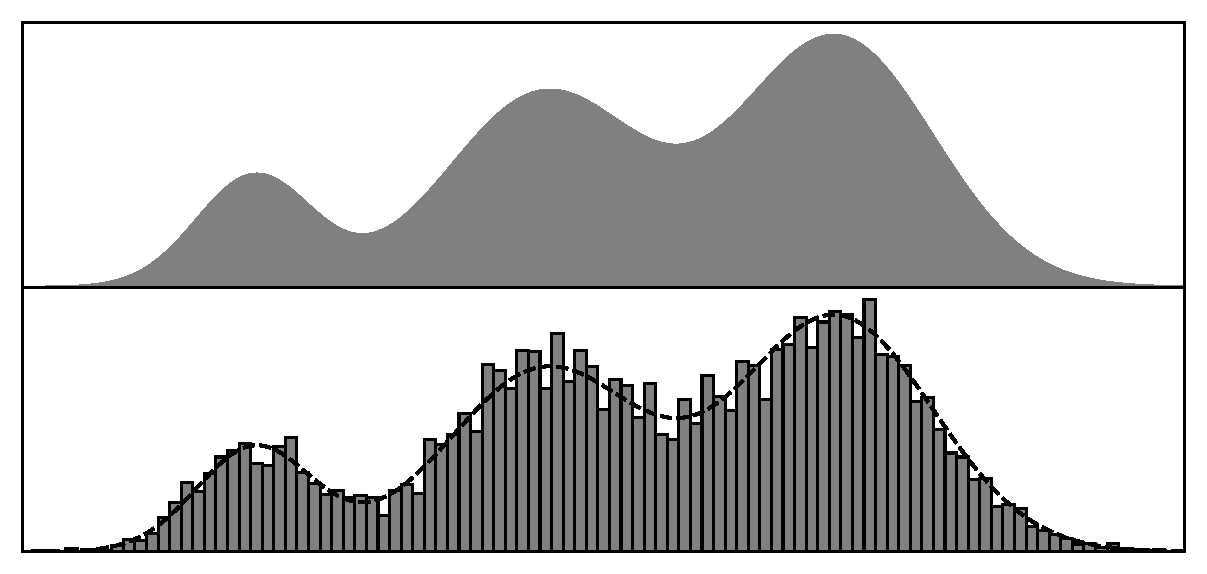
\includegraphics[width=0.7\linewidth, clip=true, trim={5mm, 2mm, 5mm, 5mm}]{inverse_cdf_transformation_method_schematic_simplified}
\caption[The inverse transform method]{The inverse transform method produces random variables following a desired pattern.}
\label{fig:inverse_cdf_transformation_method_schematic_simplified}
\end{figure}

The technical name for the expression which takes a percentile and determines what value of a random variable this corresponds to is \emph{the inverse cumulative distribution function}, sometimes called the inverse CDF or the percentage point function. Most computers and programming languages have access to these functions for some of the most popular distributions. 

\subsection{What are approximate random variables?}
\label{sec:what_are_approximate_random_variables}

So far we have painted a trouble free picture for producing random variables from whatever distribution interests us by using the inverse transform method. But suppose we have an application, such as a computer simulation, which requires lots of random variables from a distribution. As an example, it is not uncommon for financial simulations of stock markets to use anywhere from millions to trillions of random numbers to predict the value of various financial products. If this is the case, then we want to process these random numbers as quick as possible. Unfortunately, while the inverse transform method is versatile, if you do it exactly, it can be very slow and struggle to perform well on the latest hardware. This is where our research proposes the following idea: don't do it exactly, do it approximately. 

To see where we make our approximations, let's take a very important and ubiquitous distribution known as the Gaussian distribution, which is sometimes called the Normal distribution or the bell curve. The Gaussian's inverse cumulative distribution function is plotted in \Cref{fig:inverse_cdf_function_tails_simplified},
where we indicating several random positions the function might evaluate. Most of the inputs land near the centre of the function, where it's nearly a straight line and easy to evaluate. However, sometimes values land near the edges, in the more difficult shaded region where the function shoots off the edges of \Cref{fig:inverse_cdf_function_tails_simplified}, and is much harder to evaluate. While these difficult scenarios are infrequent, the greater the degree of parallelisation, the more certain it is that such values are unavoidable. It is these types of edge values which contaminate an otherwise easy calculation, leading to a loss in performance. 

\begin{figure}[htb]
\centering
\begin{subfigure}[t]{0.45\linewidth}
\centering
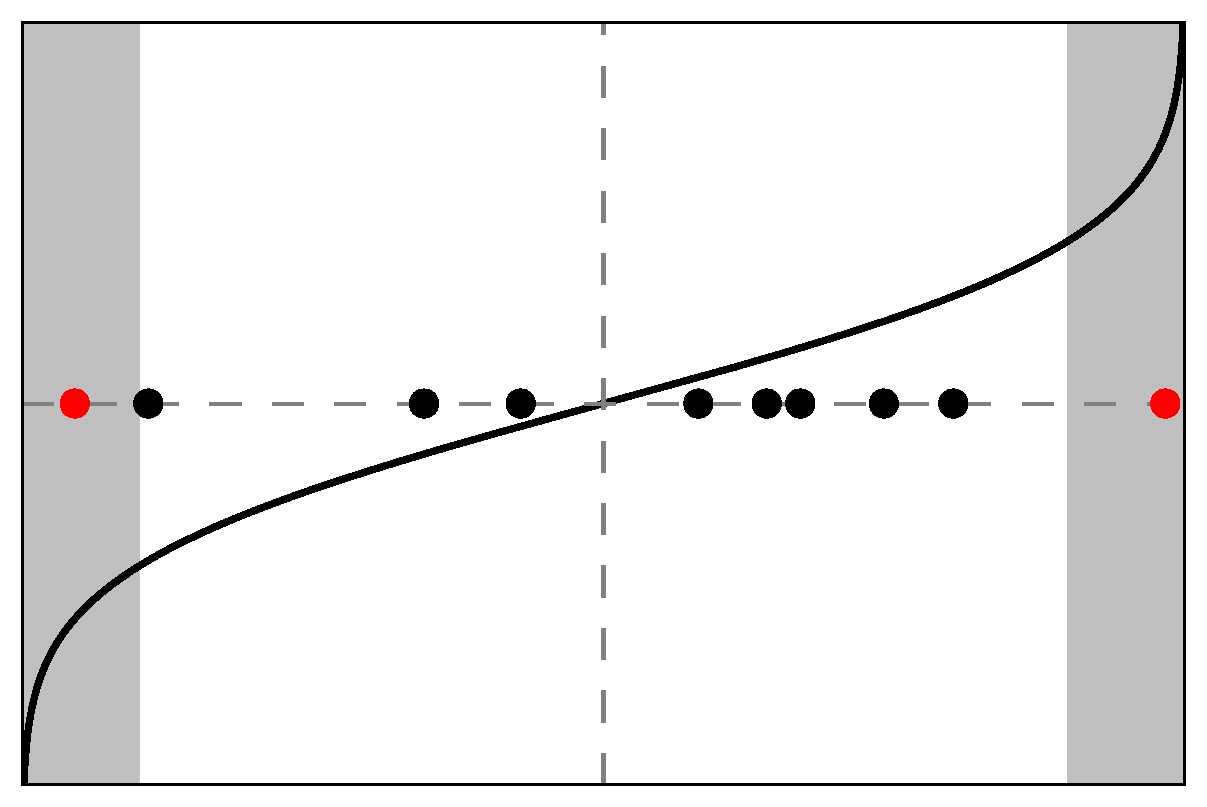
\includegraphics[width=\linewidth]{inverse_cdf_function_tails_simplified}
\begin{minipage}[t]{0.9\linewidth}
\caption{The Gaussian's inverse cumulative distribution function, and several possible random inputs (\CIRCLE). The more difficult regions are shaded, where some random inputs will unfortunately land ({\color{red}\CIRCLE})}
\label{fig:inverse_cdf_function_tails_simplified}
\end{minipage}
\end{subfigure}%
~
\begin{subfigure}[t]{0.45\linewidth}
\centering
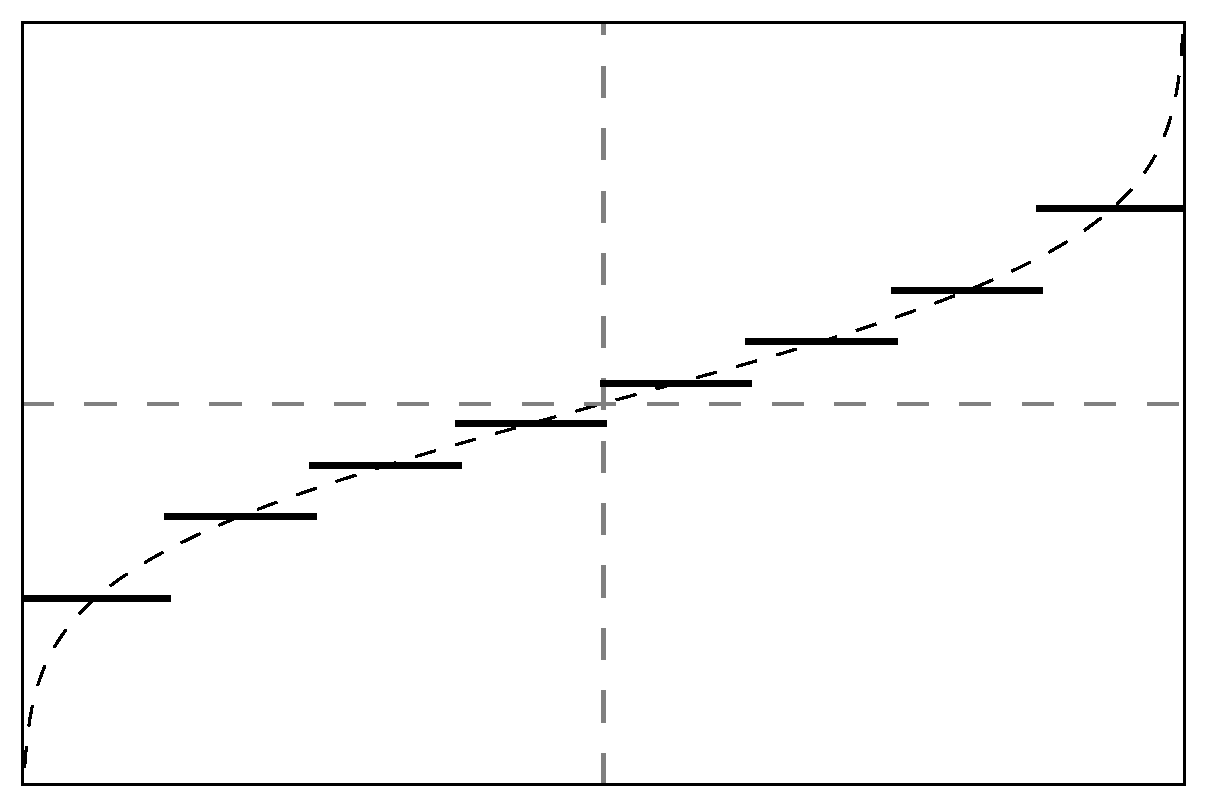
\includegraphics[width=\linewidth]{inverse_cdf_uniform_discretisation_unshaded_simplified}
\begin{minipage}[t]{0.9\linewidth}
\caption{An example approximation of the exact function. The approximation is several flat lines of equal widths.}
\label{fig:inverse_cdf_uniform_discretisation_unshaded_simplified}
\end{minipage}
\end{subfigure}
\caption{The Gaussian's inverse cumulative distribution function and an approximation.}
\label{fig:gaussian_inverse_cdf}
\end{figure}


To remedy the difficult edge cases, our research proposes introducing an approximation to the exact inverse cumulative distribution function. The approximation is designed to tackle the edge cases as easily as the central ones, and being fast irrespective of what's encountered. One example we proposed and studied was approximating the function by a series of flat lines, where an example is shown in \Cref{fig:inverse_cdf_uniform_discretisation_unshaded_simplified}. 

In our experiments, we pitted various exact implementations (some proprietary), against our approximations. Although inexact, our approximations produced random variables in a fraction of the time it takes the exact functions. The random variables produced don't exactly follow the desired distribution, but instead something very similar. When the random variables are produced  using an approximation, we call them \emph{approximate random variables}. In our research, we study the error introduced from using these instead of the exact ones. Not only can we quantify how they affect the answer, we developed a mathematical approach to counteract their error. This means we can reap the benefits of the faster speed, without losing any accuracy, getting the best of both worlds. 

\subsection{When would I use approximate random variables?}
\label{sec:when_would_i_use_approximate_random_variables}

In our research we investigated and analysed the consequences of using approximate random variables in the context of running computer simulations. This is extremely common in finance, weather forecasting, and other fields. As we mentioned, various other applications use random numbers and could likely benefit from using approximate random numbers, although there remains work to be done to investigate and analyse all of the remaining use-cases.

One particularly prolific scientific method is known as \emph{Monte Carlo}. It is heavily used for financial simulations, and requires vast quantities of random numbers, usually from the Gaussian distribution. The Monte Carlo method can be described as: run lots of simulations of whatever is of interest, compute the average of what you see, and that's approximately the answer. The more simulations you run the more accurate your answer is. 

For most people, computing averages is easy, but how does someone ``simulate''? Running a simulation is asking a computer to do the following: given where something is now, and knowing how it behaves, guess where it will be in the future? When we say we know how the system behaves, it means we have an expression which accurately describes how it will evolve. This expression though is only accurate at predicting a tiny bit into the future. To predict far into the future, one method is to split this up into lots of smaller intermediate predictions. We then predict from one step to the next, one after another, until you're at the end. 


The simplest method of simulating something step-by-step is known as the \emph{Euler scheme}, and if the evolution is subject to random influences it's the \emph{Euler-Maruyama scheme}. There are two factors influencing the evolution: one isn't random, and the other is (e.g.~traders buying and selling stocks randomly influences their price). To simulate the random bit we need a random number, and the Euler-Maruyama scheme needs them from a Gaussian distribution. Some example Euler-Maruyama simulations are shown in \Cref{fig:example_simulation}.

\begin{figure}[htb]
\centering
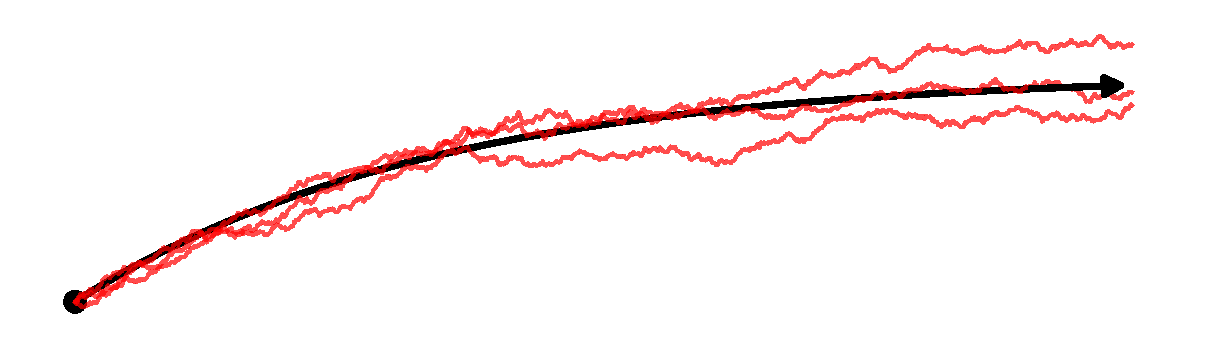
\includegraphics[width=0.7\linewidth]{example_simulation}
\caption{A non-random process (\rule[0.2em]{1.5em}{2pt}), and three Euler-Maruyama simulations ({\color{red}\rule[0.2em]{1.5em}{2pt}}).}
\label{fig:example_simulation}
\end{figure}

The Euler-Maruyama scheme is simple, a robust problem solver, and there's not much that it struggles with, so why tamper with it? One shortcoming is that at each step it requires a random number from the Gaussian distribution. Unfortunately, this is usually the most expensive bit. To give the scheme the random numbers it needs quicker, we propose swapping them for our approximate random numbers. 


Modifying the Euler-Maruyama scheme to substitute exact random numbers with approximate ones largely alleviates the bottleneck.  We can now run simulations much faster, improving the accuracy of any Monte Carlo estimate which uses the Euler-Maruyama scheme to produce the simulations. However, we cannot overlook that we compromised the quality of our simulations, and this will introducing some error into our answer. Is this significant though, or even noticeable? In our research, we've shown that the error introduced is limited in size by the error arising from approximating the Gaussian distribution. So to reduce the resulting error to an acceptable level, it's sufficient to just increase the fidelity of our approximation.

\subsection{How can I get started using them?}

All you need to get started using approximate random variables is an approximation and a problem to solve. In the code provided we will give some examples of approximating the Gaussian distribution, where we've taken some time and effort to ensure our C approximations are fast. 

Before using approximate random variables in your own setting, we encourage you go through some of the demonstrations provided to give a better idea of how to incorporate and adapt them as necessary into your own problem. We also show how one of our approximations to the Gaussian distribution can be adapted to approximate another distribution (the non-central $ \chi^2 $-distribution), and we expect our approximations can be used as templates for approximating several other distributions. 

Approximate random variables are as their name suggests: approximate. Switching to approximate random variables is easy, and can gain you huge amounts of speed. Unfortunately, swapping the exact random variables for the approximate ones and doing nothing else, while easy to code up, will introduce some error. However, with a little extra effort, by utilising a technique known as \emph{multilevel Monte Carlo}, you can counteract this error without compromising speed, and obtain the best of both worlds. This can be a little technical, and we refer a reader interested in the technicalities of the method to some of the additional material mentioned in \Cref{sec:where_can_i_learn_more}.



\clearpage
\section{The Gaussian distribution}

The bulk of our approximations have been centred on approximating Gaussian random variables, as these are used in the Euler-Maruyama scheme (and several other schemes), and the Gaussian's analytic properties are sufficiently tractable that theoretical results could be proved for our approximations. As such, we frame our discussions of approximations around   approximating the Gaussian distribution, for added utility and tractability.

\subsection{Piecewise constant approximations}

We mentioned earlier in \Cref{sec:what_are_approximate_random_variables} an approximation to the Gaussian's inverse cumulative distribution function which was comprised of a series of flat lines of equal width. The mathematical name for this approximation is a \emph{piecewise constant function} which uses \emph{equipartitioned intervals}, although we will just abbreviate this as the piecewise constant function. To construct the approximation, we first have to decide, how many intervals do we need, and what value should be use as the constant for each interval?

The number of intervals is the easy bit, so let's say we have $ N $ of them, where in most of our approximations we found $ N = 1028 $ to be sufficiently high to obtain a reasonable fidelity approximation. As for what value to use, a sensible choice is whatever you would expect to get from the exact function. The exact inverse cumulative distribution function for the Gaussian distribution is usually denoted $ \Phi^{-1} $. Denoting the start and end of a particular interval as $ a $ and $ b $ respectively, where $ a < b $, the value used for a particular interval is
\begin{equation}
\dfrac{1}{b - a}\int_a^b \Phi^{-1}(x) \dd{x} \equiv \dfrac{1}{b - a} \int_{\Phi^{-1}(a)}^{\Phi^{-1}(b)} \dfrac{z}{\sqrt{2\pi}} \exp(-\dfrac{z^2}{2}) \dd{z}.
\end{equation}
Both these integrals are equivalent to one another, where $ \Phi $ is the Gaussian's cumulative distribution function (i.e.~not the \emph{inverse} CDF, but just the CDF). Both are easy for a computer to calculate, where the second is sometimes more computationally convenient for intervals touching the edge. 

If we label the intervals $ 0, 1, 2,\ldots, N-1 $, we can store these values in an list. For a uniform random input $ U $ in the range $ 0 \leq U < 1 $, where 1 is not included, we can obtain the desired value by simply looking up the index corresponding to the relative size of $ U $ compared to $ N - 1 $. Mapping $ U $ to the index is done by multiplying by $ N $ and only keeping the integer part, and hence computes $ \lfloor U N \rfloor $, which in code can be done by something equivalent to \verb|int(U * N)|.

In the file \singlecodeline{approximate_gaussian_distribution.py} there is a function \singlecodeline{construct_piecewise_constant_approximation} which produces a piecewise constant approximation to the Gaussian's inverse cumulative distribution function. A condensed version is shown in \Cref{code:python:construct_piecewise_constant_approximation}.

\begin{lstfloat}[htb]
\begin{lstlisting}[language=python, captionpos=b, caption={Constructing a piecewise constant approximation.}, label={code:python:construct_piecewise_constant_approximation}]
def expected_value_in_interval(func, a, b):
    """ Calculates the expected value of a function inside an interval. """
    return integrate(func, a, b) / (b - a)


def build_lookup_table(func, n_table_entries):
    """ Builds a lookup table. """
    interval_width = 1.0 / n_table_entries
    lookup_table = zeros(n_table_entries)
    for n in progressbar(range(n_table_entries)):
        a = n * interval_width
        b = a + interval_width
        lookup_table[n] = expected_value_in_interval(func, a, b)
    return lookup_table


def construct_piecewise_constant_approximation(func, n_intervals):
    """ Constructs a piecewise constant approximation. """
    lookup_table = build_lookup_table(func, n_intervals)

    def piecewise_constant_approximation(u):
        """ A piecewise constant approximation. """
        return lookup_table[array(n_intervals * u).astype(int)]

    return piecewise_constant_approximation
\end{lstlisting}
\end{lstfloat}

In the file \singlecodeline{approximate_gaussian_distribution_demonstrations.py}
there is the function  
\singlecodeline{plot_piecewise_constant_approximation_of_gaussian}
which demonstrates how to use this approximation, and how you can reproduce \Cref{fig:inverse_cdf_uniform_discretisation_unshaded_simplified} for yourself. A condensed version of the function is shown in \Cref{code:python:plot_piecewise_constant_approximation_of_gaussian}, where we exclude the values 0 and 1 as the exact function struggles with these values (returning infinite values). The output from \Cref{code:python:plot_piecewise_constant_approximation_of_gaussian} is shown in \Cref{fig:piecewise_constant_approximation_of_gaussian}.

\begin{lstfloat}[htb]
\begin{lstlisting}[language=python, captionpos=b, caption={Comparing the exact and approximate functions.}, label={code:python:plot_piecewise_constant_approximation_of_gaussian}]
uniform_input = linspace(0, 1, 1000)[1:-1]  # We exclude the end points.
approximate_inverse_gaussian_cdf = \
    construct_piecewise_constant_approximation(
        inverse_gaussian_cdf, 
        n_intervals=8)
plot(uniform_input, inverse_gaussian_cdf(uniform_input))
plot(uniform_input, approximate_inverse_gaussian_cdf(uniform_input))
\end{lstlisting}
\end{lstfloat}

\begin{figure}[htb]
\centering
\includegraphics[width=0.7\linewidth]{piecewise_constant_approximation_of_gaussian}
\caption{The piecewise constant approximation produced by \Cref{code:python:plot_piecewise_constant_approximation_of_gaussian}.}
\label{fig:piecewise_constant_approximation_of_gaussian}
\end{figure}

Although the Python implementation is not optimised to be very high speed (compared to our C version), it is still much faster than the exact routine (\verb|norm.ppf| from \verb|scipy.stats|). On my machine, the function \singlecodeline{piecewise_constant_approximation_of_gaussian_timing} from the file \singlecodeline{approximate_gaussian_distribution_demonstrations.py} gives the following estimates for the average time:
\begin{verbatim}
Average time for the approximate function: 3.23281e-08 s.
Average time for the exact function: 8.69456e-07 s.
\end{verbatim}
from which we can see the approximation is approximately 30 times faster than the exact function. Of course, both of these times are much slower than equivalent C code, but it is at least indicative that there is a lot of speed to be gained. 


It is worth noting of course that the lookup table only needs to be computed once, and this can be done offline, so is not performance critical. 

So how can a higher performance version be implemented in C? Easily. Assuming we've precomputed the values for the lookup table, then these can be stored in an array, and the piecewise constant approximation is effectively a single line of C code. A slightly expanded version of the function \singlecodeline{piecewise_constant_approximation}
from the file \singlecodeline{piecewise_constant_approximation.c}
is shown in \Cref{code:c:piecewise_constant_approximation}. We can see the implementation condenses down to a single simple line of code. The reason this is so fast is because the lookup table is small enough that it will easily fit within the L2-cache. Furthermore the lookup is unconditional, and so well suited to vectorisation, and hence we explicitly mark the process as suitable for vectorisation using \verb|#pragma omp simd|.

\begin{lstfloat}[htb]
\begin{lstlisting}[style=C, captionpos=b, caption={Constructing a piecewise constant approximation.}, label={code:c:piecewise_constant_approximation}]
#include <omp.h>

#define LOOKUP_TABLE_SIZE 1024
const double lookup_table[LOOKUP_TABLE_SIZE] = {-3.37,-2.98,...,2.98,3.37};

void piecewise_constant_approximation(
    unsigned int n_samples, 
    const double *restrict input, 
    double *restrict output)
{
    #pragma omp simd
    for (unsigned int n = 0; n < n_samples; n++)
    {
        output[n] = lookup_table[(unsigned int) (LOOKUP_TABLE_SIZE * input[n])];
    }
}
\end{lstlisting}
\end{lstfloat}

To compare this against the equivalent GSL function (\verb|gsl_cdf_ugaussian_Pinv|), there is a simple series of compiler instructions in the file \singlecodeline{make_time_piecewise_constant_approximations.sh} which resembles 
\begin{verbatim}
gcc -I. -c piecewise_constant_approximation.c
gcc -I. -O0 -c time_piecewise_constant_approximations.c
gcc -I. -o time_piecewise_constant_approximations [object_files] -lgsl
\end{verbatim}
and produces the executable \singlecodeline{time_piecewise_constant_approximations}

On my machine, which is not vector capable, and running with minimal optimisations, we obtain
\begin{verbatim}
Average time for the approximate function: 2.28712e-09 s.
Average time for the exact (GSL) function: 2.18994e-08 s.
\end{verbatim}
Similar to before the approximation is 10 times faster than the exact function from GSL, without any optimisation. Furthermore, both functions are running 10 times faster in C than in Python, which is not too surprising. If we compile \singlecodeline{piecewise_constant_approximation.c}
under \verb|-O3| then this changes to 
\begin{verbatim}
Average time for the approximate function: 9.3289e-10 s.
Average time for the exact (GSL) function: 2.18471e-08 s.
\end{verbatim}
widening the speed increase to nearly 25 times. With vector capable hardware and some fine tuning with OpenMP, the method can be very competitive. 


Moving this onto some \intel Skylake AVX512 hardware and compiling using 
\begin{verbatim}
icc -I. -std=c11 -O3 -simd -p -mkl -qopenmp -xCORE-AVX512 \
    -march=skylake-avx512 -qopt-zmm-usage=high -c \
    piecewise_constant_approximation.c 
icc -I. -mkl -O0 -c time_piecewise_constant_approximation.c \
    -D__PURE_INTEL_C99_HEADERS__
icc -I. -o time_piecewise_constant_approximation [object_files] \
    -lgsl -lgslcblas
\end{verbatim}
our simple implementation does okay, achieving
\begin{verbatim}
Average time for the approximate function: 8.9733e-10 s.
Average time for the exact (GSL) function: 2.2618e-08 s.
\end{verbatim}
and when this is adapted to use \verb|-DUSE_VECTOR_BATCHES| (see the makefile and source code for an explanation) this improves to
\begin{verbatim}
Average time for the approximate function: 7.5127e-10 s.
Average time for the exact (GSL) function: 2.26445e-08 s.
\end{verbatim}
which corresponds to about 1.7 clock-cycles on average (the machine runs at \SI{2.3}{\giga\hertz}), in keeping with the findings from previous work. 



\subsection{Piecewise polynomial approximations}


There are a few natural ways to extend the piecewise constant approximation, and the two most obvious are: increase the order of the polynomial, and change the spacing of the intervals so they're denser around the edges. 

Starting with increasing the order of the polynomial, the next improvement from a piecewise constant is a piecewise linear function. So the next question is which linear function best approximates the function in a given interval. There are various measures of the error, including the worse case error, or the average case error. For Monte Carlo applications, we used a variant called \emph{the mean squared error}, known mathematically as \emph{the $ L^2 $-error} (some definitions use the \emph{root mean squared error}). One of the advantages of the $ L^2 $-error, is that it is relatively easy to determine the optimal parameters. For a function $ f $, let's approximate this using a function $ \tilde{f} $, where we write it as an $ m $-th order polynomial  
\begin{equation}
f(u) \approx \tilde{f}(u) = c_0 + c_1 u + c_2 u^2 + \cdots + c_m u^m. 
\end{equation}
So how can we determine the optimal coefficients? The error can be expressed as 
\begin{equation}
\int_{a}^{b} \parens{f(u) - \sum_{i=0}^{m}c_i u^i}^2 \dd{u}.
\end{equation}
We can minimise this by differentiating with respect to each coefficient $ c_i $ and finding the values which make the derivative zero. Doing this for each of the coefficients, we obtain the set of $ m + 1 $ simultaneous equations 
\begin{equation}
\sum_{i=0}^{m} c_i \parens{\dfrac{b^{i+j+1} - a^{i + j + 1}}{i + j + 1}} = \int_{a}^{b} u^j f(u) \dd{u}
\end{equation}
for $ j = 0,1,2,\ldots,m $, which is equivalent to an equation of the form 
\begin{equation}
A\bm{x} = \bm{b}.
\end{equation} 
Luckily, solving simultaneous equations of this form is easy for computers, and so the coefficients are easily determined, where 
\begin{gather}
\bm{b}_i = \int_{a}^{b} u^i f(u) \dd{u} \\
\shortintertext{and}
A_{i,j} = \dfrac{b^{i+j+1} - a^{i + j + 1}}{i + j + 1}, \\
\shortintertext{and we are solving for values of $ \bm{x} $, where}
\bm{x}_i = c_i.
\end{gather}

The improvement we also want to make is to make the intervals denser near the edges of the function, as these are the trickiest bits which require the most effort from an approximation. One way to achieve this is to have the intervals geometrically decaying in size near the edge, and one decay rate which is particularly well suited for computer calculations is in powers of two (as computers work in binary). When the intervals are decaying powers of two, we give these the special name of \emph{dyadic intervals}.

All inverse cumulative distribution functions are defined for valued between 0 and 1, and so we only need dyadic intervals in this range. If we again consider $ N $ intervals in this range, each corresponding to an index, they are as shown in \Cref{tab:dyadic_intervals_array_indices}.

\begin{table}[htb]
\centering
\begin{tabular}{cc}
Dyadic interval         & Index \\ \hline
$ [\tfrac{1}{2}, 1) $           &          0           \\
$ [\tfrac{1}{4}, \tfrac{1}{2}) $     &          1           \\
$ [\tfrac{1}{8}, \tfrac{1}{4}) $     &          2           \\
$ \vdots $                &      $ \vdots $      \\
$ [\tfrac{1}{2^{n+1}}, \tfrac{1}{2^n}) $ &        $ n $ \\
$ \vdots $                &      $ \vdots $      \\
$ [0, \tfrac{1}{2^{N-1}}) $ &        $ N-1 $
\end{tabular}
\caption{The indices for various dyadic intervals.}
\label{tab:dyadic_intervals_array_indices}
\end{table}

These intervals are dense near zero, but they are not dense near 1. Is this a problem? Not really. For the Gaussian's inverse cumulative distribution function, this is rotationally symmetric about $ \tfrac{1}{2} $ such that $ \Phi^{-1}(U) \equiv -\Phi^{-1}(1-U) $, and so values near one are easily computed by the equivalent value reflected about $ \tfrac{1}{2} $. Notice that if we reflect about $ \tfrac{1}{2} $, then there will be one interval, the 0 index interval, which will contain just the one value $ \tfrac{1}{2} $. While this is a slight computational redundancy, ensuring this value has an interval in which it belongs ensures any approximation won't break if it is given the perfectly valid value of $ \tfrac{1}{2} $.

Taking an order~1 polynomial, corresponding to a piecewise linear function, in the file \singlecodeline{approximate_gaussian_distribution.py} the function \singlecodeline{construct_symmetric_piecewise_polynomial_approximation} provides a relatively simple demonstration of how to build and implement such a function. A small demonstration of how to use this can be found in function \singlecodeline{plot_piecewise_polynomial_approximation_of_gaussian} from \singlecodeline{approximate_gaussian_distribution_demonstrations.py}
where the output is shown in \Cref{fig:piecewise_polynomial_approximation_of_gaussian}. If the number of intervals in increased to a modest amount (e.g.~8 or 16) then the approximation achieves a very high fidelity very quickly. In \Cref{fig:piecewise_polynomial_approximation_of_gaussian} we only use a very small number of intervals, else the approximation and the exact function would be indistinguishable.

\begin{figure}[htb]
\centering
\includegraphics[width=0.7\linewidth]{piecewise_polynomial_approximation_of_gaussian}
\caption{A piecewise linear approximation using dyadic intervals.}
\label{fig:piecewise_polynomial_approximation_of_gaussian}
\end{figure}

It is worth noting that the Python implementation provided in 
\singlecodeline{approximate_gaussian_distribution_demonstrations.py}
is only demonstrative, but is not particularly high performance, where the function \singlecodeline{piecewise_constant_polynomial_of_gaussian_timing}
produces
\begin{verbatim}
Average time for the exact function: 8.93741e-08 s.
Average time for the approximate function: 1.22783e-06 s.
\end{verbatim}
showing that our Python implementation is approximately 15 times slower than the exact function! (It will be our C implementations which will be fast). 

To get an idea of how accurate these approximations are for different numbers of intervals and varying polynomial orders, the function \singlecodeline{plot_error_of_piecewise_polynomial_approximation_of_gaussian} computes the RMSE for various configurations, with the results shown in \Cref{fig:piecewise_polynomial_approximation_of_gaussian_rmse}.

\begin{figure}[htb]
\centering
\includegraphics[width=0.7\linewidth]{piecewise_polynomial_approximation_of_gaussian_rmse}
\caption{Error of piecewise polynomial approximations.}
\label{fig:piecewise_polynomial_approximation_of_gaussian_rmse}
\end{figure}

We are not particularly discouraged by this Python result, as this approximation can be extremely performant on vector hardware, assuming a sufficiently wide vector length. The reason for this is simple, let us suppose we are working in 32-bit single-precision, and we are using the reasonably high fidelity 16-interval piecewise cubic approximation. If we store the possible coefficients for a given term in a list, then this will only require 512-bits ($ 32 \times 16 = 512 $), which is the vector width on a lot of modern hardware, such as \intel's AVX512 Skylake hardware or newer. This means that when we lookup the coefficients for a given term, instead of querying the cache, we can query a vector register, where we will only need 4 vector registers to hold all the coefficients we need. Additionally, if we are using dyadic intervals, then we can easily determine the index by reading the exponent bits of the floating-point number using bit-wise operations (much quicker than how we did this in Python). This all means we never even need to look in the cache, everything we require is held in vector registers, and we only need a few simple arithmetic operations (which can even use FMAs) and bit manipulations. This means that a C implementation can achieve very high speeds.

In the file \singlecodeline{piecewise_polynomial_approximation.c} we provide several implementations of a piecewise polynomial approximation using the function \singlecodeline{piecewise_polynomial_approximation}
where there several implementations targeting different architectures. Different implementations are compiled depending on the value of various macro definitions passed to the compiler (using ``\verb|-D|<macro-name>''), as described in \Cref{tab:piecewise_polynomial_approximation_implementations}. To use a cubic approximation implemented using OpenMP you would compile with the flags
\singlecodeline{-DUSE_OPENMP_SIMD_APPROX -DPOLYNOMIAL_ORDER=3}

\begin{table}[htb]
\centering
\begin{tabular}{lllc}
Macro & Target & Vectors &  \verb|POLYNOMIAL_ORDER| \\
\hline
\verb|USE_OPENMP_SIMD_APPROX|  & Any & Any & 1, 3\\
\verb|USE_INTEL_INTRINSICS_APPROX_CUBIC| & Intel & AVX512& 3\\
\verb|USE_INTEL_INTRINSICS_APPROX_LINEAR| &Intel &  AVX512 & 1\\
\verb|USE_ARM_SVE_INLINE_APPROX_CUBIC| & Arm & SVE 512-bits & 3 \\
\end{tabular}
\caption{Piecewise polynomial approximation implementations.}
\label{tab:piecewise_polynomial_approximation_implementations}
\end{table} 

All of the implementations are written assuming IEEE 32-bit single-precision floats, require 16 dyadic intervals, and assume vector widths of 512-bits (even for SVE). Our set of implementations is not complete nor exhaustive, and there is likely some room for more fine tuning and optimisation. Nonetheless, some can be readily copied, while we hope that others serve as useful templates for constructing other approximations. 

Some condensed versions of these implementations (with most of the comments removed for brevity) are shown in \Cref{code:c:piecewise_polynomial_approximation_use_openmp_simd_approx,code:c:piecewise_polynomial_approximation_use_arm_sve_inline_approx_cubic,code:c:piecewise_polynomial_approximation_use_intel_intrinsics_approx_cubic}, demonstrating an OpenMP SIMD implementation, an \arm SVE implementation, and an \intel intrinsics implementation. An explanation of what is going on in each of these implementations is provided in \Cref{algo:piecewise_polynomial_approx_using_dyadic_intervals}.

\begin{algorithm}[H]
\DontPrintSemicolon
\KwIn{Floating-point uniform random number $ U \in [0, 1) $.}
\KwOut{Floating-point piecewise polynomial approximation.}
Form predicate based on whether $ U > \tfrac{1}{2} $.\;
Reflect about $ \tfrac{1}{2} $ to obtain $ U \in [0, \tfrac{1}{2}] $.\;
Alias $ U $ as an unsigned integer.\;
Read the exponent bits using bitwise-AND.\;
Right shift away the mantissa's bits.\;
Obtain an array index by correcting for exponent bias.\;
Cap the array index to avoid overflow.\;
Read the polynomial coefficients using the array index.\;
Re-interpret $ U $ as a float.\;
Form the polynomial approximation.\;
Correct sign of approximation based on predicate.\;
\caption[Piecewise polynomial approximation using dyadic intervals]{Piecewise polynomial approximation using dyadic intervals.}
\label{algo:piecewise_polynomial_approx_using_dyadic_intervals}
\end{algorithm}

\begin{lstfloat}[H]
\begin{lstlisting}[style=C, captionpos=b, caption={Piecewise polynomial approximation implementations using OpenMP.}, label={code:c:piecewise_polynomial_approximation_use_openmp_simd_approx}]
#include "piecewise_polynomial_approximation.h"
#include "piecewise_polynomial_approximation_coefficients.h"

// For IEEE 754
#define N_MANTISSA_32 23
#define FLOAT32_EXPONENT_BIAS 127
#define FLOAT32_EXPONENT_BIAS_TABLE_OFFSET (FLOAT32_EXPONENT_BIAS - 1)
#define TABLE_MAX_INDEX (TABLE_SIZE - 1) // Zero indexing...
#define FLOAT32_AS_UINT32(x) (*((uint32 *) &x))  // Type-punning is performed.

#pragma omp declare simd
static inline float32 polynomial_approximation(float32 u, uint32 b);

#pragma omp declare simd
static inline uint32 get_table_index_from_float_format(float32 u);

static inline float32 polynomial_approximation(float32 u, uint32 b) 
{
    #if (POLYNOMIAL_ORDER == 3)
    float32 z, z_even, z_odd;
    float32 x = u * u;
    z_even = poly_coef_0[b] + poly_coef_2[b] * x;
    z_odd = poly_coef_1[b] + poly_coef_3[b] * x;
    z = z_even + z_odd * u;
    return z;
    #elif (POLYNOMIAL_ORDER == 1)
    float32 z =  poly_coef_0[b] + poly_coef_1[b] * u;
    return z;
    #else
    #endif
}

static inline uint32 get_table_index_from_float_format(float32 u)
{
    uint32 b;
    b = FLOAT32_AS_UINT32(u) >> N_MANTISSA_32; // Keeping only the exponent.
    b = FLOAT32_EXPONENT_BIAS_TABLE_OFFSET - b; // Getting the table index.
    b = b > TABLE_MAX_INDEX ? TABLE_MAX_INDEX : b;  // Avoiding overflow.
    return b;
}

#ifdef USE_OPENMP_SIMD_APPROX
void piecewise_polynomial_approximation(
    unsigned int n_samples,
    const float32 *restrict input, 
    float32 *restrict output)
{
    #pragma omp simd 
    for (unsigned int i = 0; i < n_samples; i++)
    {
        float32 u, z;
        u = input[i];
        bool predicate = u < 0.5f;
        u = predicate ? u : 1.0f - u;
        uint32 b = get_table_index_from_float_format(u);
        z = polynomial_approximation(u, b);
        z = predicate ? z : -z;
        output[i] = z;
    }
}
#endif
\end{lstlisting}
\end{lstfloat}

\begin{lstfloat}[H]
\begin{lstlisting}[style=C, captionpos=b, caption={Piecewise polynomial approximation implementations using \arm SVE inline assembly.}, label={code:c:piecewise_polynomial_approximation_use_arm_sve_inline_approx_cubic}]
// This is not VLA, but assumes vector lengths sufficient to hold the arrays.
#ifdef USE_ARM_SVE_INLINE_APPROX_CUBIC
void piecewise_polynomial_approximation(unsigned int n_samples, 
    const float32 *restrict input, float32 *restrict output)
{
    unsigned int i;  // A dummy variable.
    asm (""
        "\tcbz %[n_samples], 2f                                     "  
        "\n\tmov %[i], xzr                                          "
        "\n\tfmov    z0.s, #5.000000000000000000e-01                "
        "\n\tptrue   p0.s                                           "
        "\n\tfmov    z1.s, #1.000000000000000000e+00                "
        "\n\tld1w    {z2.s}, p0/z, [%[poly_coef_0], %[i], lsl #2]   "
        "\n\tld1w    {z3.s}, p0/z, [%[poly_coef_1], %[i], lsl #2]   "
        "\n\tld1w    {z4.s}, p0/z, [%[poly_coef_2], %[i], lsl #2]   "
        "\n\tld1w    {z5.s}, p0/z, [%[poly_coef_3], %[i], lsl #2]   "
        "\n\tmov z6.s, #126                                         "
        "\n\tmov z7.s, %[table_max_index]                           "
        "\n\twhilelo p1.s, xzr, %[n_samples]                        "
        "\n1:                                                       "
        "\n\tld1w    {z8.s}, p1/z, [%[input], %[i], lsl #2]         "
        "\n\tfsub    z9.s, z1.s, z8.s                               "
        "\n\tfcmgt   p2.s, p0/z, z0.s, z8.s                         "
        "\n\tsel z8.s, p2, z8.s, z9.s                               "
        "\n\tlsr z9.s, z8.s, #23                                    "
        "\n\tsub z9.s, z6.s, z9.s                                   "
        "\n\tcmplo   p3.s, p0/z, z9.s, %[table_max_index]           "
        "\n\tsel z9.s, p3, z9.s, z7.s                               "
        "\n\tfmul    z10.s, z8.s, z8.s                              "
        "\n\ttbl z11.s, {z2.s}, z9.s                                "
        "\n\ttbl z12.s, {z4.s}, z9.s                                "
        "\n\tfmad    z12.s, p0/m, z10.s, z11.s                      "
        "\n\ttbl z11.s, {z3.s}, z9.s                                "
        "\n\ttbl z13.s, {z5.s}, z9.s                                "
        "\n\tfmad    z13.s, p0/m, z10.s, z11.s                      "
        "\n\tfmad    z13.s, p0/m, z8.s, z12.s                       "
        "\n\tfneg    z10.s, p0/m, z13.s                             "
        "\n\tsel z10.s, p2, z13.s, z10.s                            "
        "\n\tst1w    {z10.s}, p1, [%[output], %[i], lsl #2]         "
        "\n\tincw    %[i]                                           "
        "\n\twhilelo p1.s, %[i], %[n_samples]                       "
        "\n\tb.any 1b                                               "
        "\n2:                                                       "
        "\n\t                                                       "
        : [i] "=&r" (i) 
        : "[i]" (0), [input] "r" (input), [output] "r" (output),
        [n_samples] "r" (n_samples), [poly_coef_0] "r" (poly_coef_0),
        [poly_coef_1] "r" (poly_coef_1), [poly_coef_2] "r" (poly_coef_2),
        [poly_coef_3] "r" (poly_coef_3), [table_max_index] "i" (TABLE_MAX_INDEX)
        : "memory", "cc", "p0", "p1", "p2", "p3", "z0", "z1", "z2", "z3", "z4",
        "z5", "z6", "z7", "z8", "z9", "z10", "z11", "z12", "z13"
        );
}
#endif
\end{lstlisting}
\end{lstfloat}

\begin{lstfloat}[H]
\begin{lstlisting}[style=C, captionpos=b, caption={Piecewise polynomial approximation implementations using \intel intrinsics.}, label={code:c:piecewise_polynomial_approximation_use_intel_intrinsics_approx_cubic}]
// Using AVX512 intrinsics. 
#ifdef USE_INTEL_INTRINSICS_APPROX_CUBIC
void piecewise_polynomial_approximation(unsigned int n_samples, 
    const float32 *restrict input, float32 *restrict output)
{
    unsigned int n_iterations = n_samples / VECTOR_LENGTH;  
    /* Loading in the constants. */
    __m512 half_float = _mm512_set1_ps(0.5f);
    __m512 one_float = _mm512_set1_ps(1.0f);
    __m512 minus_zero_float = _mm512_set1_ps(-0.0f);  // For negation.
    __m512i exponent_bias_table_offset = 
        _mm512_set1_epi32(FLOAT32_EXPONENT_BIAS_TABLE_OFFSET);
    __m512i table_max_index = _mm512_set1_epi32(TABLE_MAX_INDEX);
    __m512 coef_0 = _mm512_load_ps(poly_coef_0);  
    __m512 coef_1 = _mm512_load_ps(poly_coef_1);
    __m512 coef_2 = _mm512_load_ps(poly_coef_2);
    __m512 coef_3 = _mm512_load_ps(poly_coef_3);
    __m512 c_0, c_1, c_2, c_3;
    __m512i c;  // A useful temporary variable.
    __m512 u, z, z_even, z_odd, u_squared;
    __m512i b;
    for (int i = 0, offset = 0; i < n_iterations; i++, offset += VECTOR_LENGTH)
    {
        // Loading in the data.
        u = _mm512_loadu_ps(input + offset);
        // Forming the predicate.
        __mmask16 predicate = _mm512_cmplt_ps_mask(half_float, u);
        // Transforming the input to [0, 0.5].
        u = _mm512_mask_sub_ps(u, predicate, one_float, u);
        b = _mm512_castps_si512(u);  
        // Getting the indices.
        b = _mm512_srli_epi32(b, N_MANTISSA_32);
        b = _mm512_sub_epi32(exponent_bias_table_offset, b);
        b = _mm512_min_epi32(b, table_max_index);
        // Obtaining the relevant coefficients.
        c = _mm512_castps_si512(coef_0);
        c = _mm512_permutexvar_epi32(b, c);
        c_0 = _mm512_castsi512_ps(c);
        c = _mm512_castps_si512(coef_1);
        c = _mm512_permutexvar_epi32(b, c);
        c_1 = _mm512_castsi512_ps(c);
        c = _mm512_castps_si512(coef_2);
        c = _mm512_permutexvar_epi32(b, c);
        c_2 = _mm512_castsi512_ps(c);
        c = _mm512_castps_si512(coef_3);
        c = _mm512_permutexvar_epi32(b, c);
        c_3 = _mm512_castsi512_ps(c);
        // Building the polynomial.
        u_squared = _mm512_mul_ps(u, u);
        z_even = _mm512_fmadd_ps(c_2, u_squared, c_0);
        z_odd = _mm512_fmadd_ps(c_3, u_squared, c_1);
        z = _mm512_fmadd_ps(z_odd, u, z_even);
        z = _mm512_mask_xor_ps(z, predicate, minus_zero_float, z); // Negation.
        // Writing the result.
        _mm512_storeu_ps(output + offset, z);
    }
}
#endif
\end{lstlisting}
\end{lstfloat}
\clearpage

On my personal scalar machine, compiling the \openmp SIMD version using \singlecodeline{make_time_piecewise_polynomial_approximations.sh} 
which for a piecewise cubic approximation looks like
\begin{verbatim}
gcc -I. -fopenmp -Ofast -DUSE_OPENMP_SIMD_APPROX -DPOLYNOMIAL_ORDER=3 \
    -c piecewise_polynomial_approximation.c
gcc -I. -O0 -c time_piecewise_polynomial_approximation.c
gcc -I. -o time_piecewise_polynomial_approximation [object_files] -lgsl
\end{verbatim}
I obtain
\begin{verbatim}
Average time for the approximate function: 5.5168e-09 s.
Average time for the exact (GSL) function: 2.2597e-08 s.
\end{verbatim}
GSL is as expected, and the SIMD cubic is slightly slower than the piecewise constant. Given the scalar hardware, this is not too surprising. 

Moving onto an \intel machine\footnote{\verb|lscpu| gives \verb|Intel(R) Xeon(R) Gold 6140 CPU @ 2.30GHz|.} we can inspect the performance of the C implementations using AVX512 intrinsics. Building a cubic approximation using
\begin{verbatim}
icc -I.  -DUSE_INTEL_INTRINSICS_APPROX_CUBIC -DPOLYNOMIAL_ORDER=3 \
    -std=c11 -O3 -simd -p -mkl -qopenmp -xCORE-AVX512 \
    -march=skylake-avx512 -qopt-zmm-usage=high -c \
    piecewise_polynomial_approximation.c 
icc -I. -mkl -O0 -c time_piecewise_polynomial_approximation.c \
    -D__PURE_INTEL_C99_HEADERS__
icc -I. -o time_piecewise_polynomial_approximation \
    [object_files] -lgsl -lgslcblas
\end{verbatim}
we obtain the executable
\singlecodeline{time_piecewise_polynomial_approximation} 
where for the piecewise linear function we instead use the flags \singlecodeline{ -DUSE_INTEL_INTRINSICS_APPROX_LINEAR -DPOLYNOMIAL_ORDER=1}
the cubic obtains
\begin{verbatim}
Average time for the approximate function: 3.93652e-10 s.
Average time for the exact (GSL) function: 2.70001e-08 s.
\end{verbatim}
and the linear obtains
\begin{verbatim}
Average time for the approximate function: 2.49551e-10 s.
Average time for the exact (GSL) function: 2.6856e-08 s.
\end{verbatim}
We can see that at a frequency of \SI{2.3}{\giga\hertz} these correspond to average times of 0.9 and 0.6 clock-cycles per input, which is in keeping with our previous research, and is very fast. 

These C implementations are designed to be fast and high performance. Nonetheless, we are sure with some more profiling, trying some other compiler flags, and perhaps a bit more effort they may yet yield a bit more performance. It is worth noting that our approximations are much faster than the exact functions from \intel's MKL, which can be included in our comparisons using the flag \singlecodeline{-DCOMPARE_AGAINST_MKL} when compiling \singlecodeline{time_piecewise_polynomial_approximation.c}
and gives the results
\begin{verbatim}
Average time for the approximate function: 2.13887e-10 s.
Average time for the exact (GSL) function: 2.40896e-08 s.
Average time for the exact (Intel HA) function: 2.93076e-09 s.
Average time for the exact (Intel LA) function: 2.16174e-09 s.
\end{verbatim}
where not only is our approximation averaging around 0.5 clock-cycles, it is around 10 times faster than \intel. 

At the time of writing, SVE capable hardware is in the preliminary stages of release, and we don't currently have access to a machine. However, to enable SVE compilation we recommend exploring the follow flags for \verb|armclang|: \singlecodeline{-armpl -fsimdmath -fvectorize -march=armv8.4-a+sve -mcpu=thunderx2t99}
amongst several others. 

\clearpage
\section{The non-central $ \chi^2 $-distribution}

The non-central $ \chi^2 $-distribution $ \chi^2_\nu(\lambda) $ with $ \nu $ degrees of freedom and non-centrality parameter $ \lambda $ is another common distribution, where $ \nu > 0 $ and $ \lambda \geq 0 $. One application of note where this occurs is the Cox-Ingersoll-Ross (CIR) model for interest rates. The inverse cumulative distribution function for this distribution, which we call $ C^{-1}_{\nu}(\cdot;\lambda) $ is very expensive to calculate, where the results from a relative comparison to the Gaussian are shown in \Cref{tab:non_central_chi_2_times}. Although there are two parameters, $ \nu $ and $ \lambda $, for a simulation with a constant time increment $ \nu $ is a constant, and so $ C^{-1}_{\nu}(\cdot;\lambda) $ can be regarded as only being parametrised by $ \lambda $. Thus we need to build a parametrised approximation. 

\begin{table}[htb]
    \centering
    \hfill
    \noindent
    \begin{subtable}[t]{0.4\linewidth}
    \centering    
    \begin{tabular}{|r|rrrrr|}
    \multicolumn{1}{c}{\multirow{2}{*}{$ \lambda $}} & \multicolumn{5}{c}{$ \nu $} \\
    \cline{2-6}
    \multicolumn{1}{c|}{} & 1 &   5  &  10 &  50  & 100 \\
    \hline
    1    &  37 &  36 &  40 &  54 &  73\\
    5    &  40 &  46 &  48 &  62 &  85\\
    10   &  54 &  56 &  63 &  69 &  97\\
    50   & 101 & 103 & 103 & 144 & 143\\
    100  & 191 & 190 & 192 & 189 & 185\\
    200  & 243 & 246 & 240 & 233 & 221\\
    500  & 465 & 474 & 465 & 446 & 416\\
    1000 & 459 & 458 & 455 & 471 & 474 \\
    \hline
\end{tabular}\\[1em]
\begin{minipage}[t]{0.9\linewidth}
\caption{Using Python and \texttt{ncx2.ppf} from Scipy's \texttt{scipy.stats}.}
\label{tab:non_central_chi_2_times_python}
\end{minipage}
\end{subtable}
\hfill
\begin{subtable}[t]{0.55\linewidth}   
    \centering     
    \begin{tabular}{|r|rrrrr|}
    \multicolumn{1}{c}{\multirow{2}{*}{$ \lambda $}} & \multicolumn{5}{c}{$ \nu $} \\
    \cline{2-6}
    \multicolumn{1}{c|}{} & 1 &   5  &  10 &  50  & 100 \\
    \hline
    1& 168 & 214 & 259 & 456 & 294  \\ 
    5& 651 & 782 & 840 & 1510 & 2046  \\ 
    10& 935 & 1086 & 1050 & 1838 & 2496  \\ 
    50& 3000 & 2969 & 2562 & 4118 & 5333  \\ 
    100& 4929 & 3461 & 5039 & 6046 & 6299  \\ 
    200& 9456 & 9603 & 10129 & 11524 & 12766  \\ 
    500& 22691 & 22713 & 22702 & 23328 & 26273  \\ 
    1000& 45872 & 43968 & 43807 & 44563 & 46780  \\
    \hline
\end{tabular}\\[1em]
\begin{minipage}[t]{0.9\linewidth}
    \caption{Using MATLAB and \texttt{ncx2inv} from MATLAB's statistics and machine learning toolbox.}
    \label{tab:non_central_chi_2_times_matlab}
\end{minipage}
\end{subtable}
\hfill
\caption[Computational times for inverse non-central $ \chi^2 $ cumulative distribution]{The ratio of average computational times for evaluating the inverse non-central $ \chi^2 $ cumulative distribution function against the inverse Gaussian cumulative distribution function for several values of the non-centrality parameter $ \lambda $ and degrees of freedom $ \nu $.}
\label{tab:non_central_chi_2_times}
\end{table}

You can generate the results from \Cref{tab:non_central_chi_2_times} yourself in MATLAB and Python. For MATLAB run the file \singlecodeline{non_central_chi_squared.m} to obtain
\begin{verbatim}
	               nu
        ------------------------------
lambda  |1      5       10      50 	
--------------------------------------
1       | 182   213     267     431 	
5       | 136   675     801     1382 	
10      | 927   879     951     1756 	
50      | 2815  2009    2690    3946 	
100     | 4951  5179    4781    6700 	
200     | 9639  8702    9539    11054 	
\end{verbatim} 
and for Python run the file \singlecodeline{non_central_chi_squared.py} to obtain
\begin{verbatim}
nu       1    5    10   50
lambda                    
1        33   40   42   57
5        43   50   50   63
10       55   58   66   74
50      105  108  108  151
100     196  172  196  203
200     248  252  250  245
\end{verbatim}


It is not particularly wise to try and directly approximate the inverse cumulative distribution function $ C^{-1}_{\nu}(\cdot;\lambda) $, as it is not particularly well scaled for various values of its parameters. Instead, if we define the function $ P_x(\cdot;y) $ as 
\begin{equation}
P_x(U;y) \coloneqq \sqrt{\dfrac{x}{4y}}\parens{ \dfrac{y}{x}  C^{-1}_{x}\parens{U; \dfrac{(1 - y)x}{y}} - 1}
\end{equation}
for $ x > 0 $ and $ 0 < y < 1  $, then we have 
\begin{equation}
C^{-1}_{\nu}(U;\lambda) = \lambda + \nu + 2 \sqrt{\lambda + \nu} P_\nu\parens{U;\dfrac{\nu}{\lambda + \nu}}.
\end{equation}
The reason this is preferable is because $ P_x(\cdot;y) $ is much better scaled for the range of possible parameters, where it has the limits
\begin{align}
P_x(U;y) & \xrightarrow{y\to 0} \Phi^{-1}(U) \\
\shortintertext{and}
P_x(U;y) & \xrightarrow{y\to 1} \dfrac{C^{-1}_x(U)}{2\sqrt{x}} - \dfrac{\sqrt{x}}{2},
\end{align}
where $ C^{-1}_\nu $, without the parameter $ \lambda $, is the inverse cumulative distribution function of the central $ \chi^2 $-distribution. We can see its convergence to these two limits in \Cref{fig:cir_update_factor_convergence_to_gaussian_both_limits}.

\begin{figure}[h!tb]
\centering
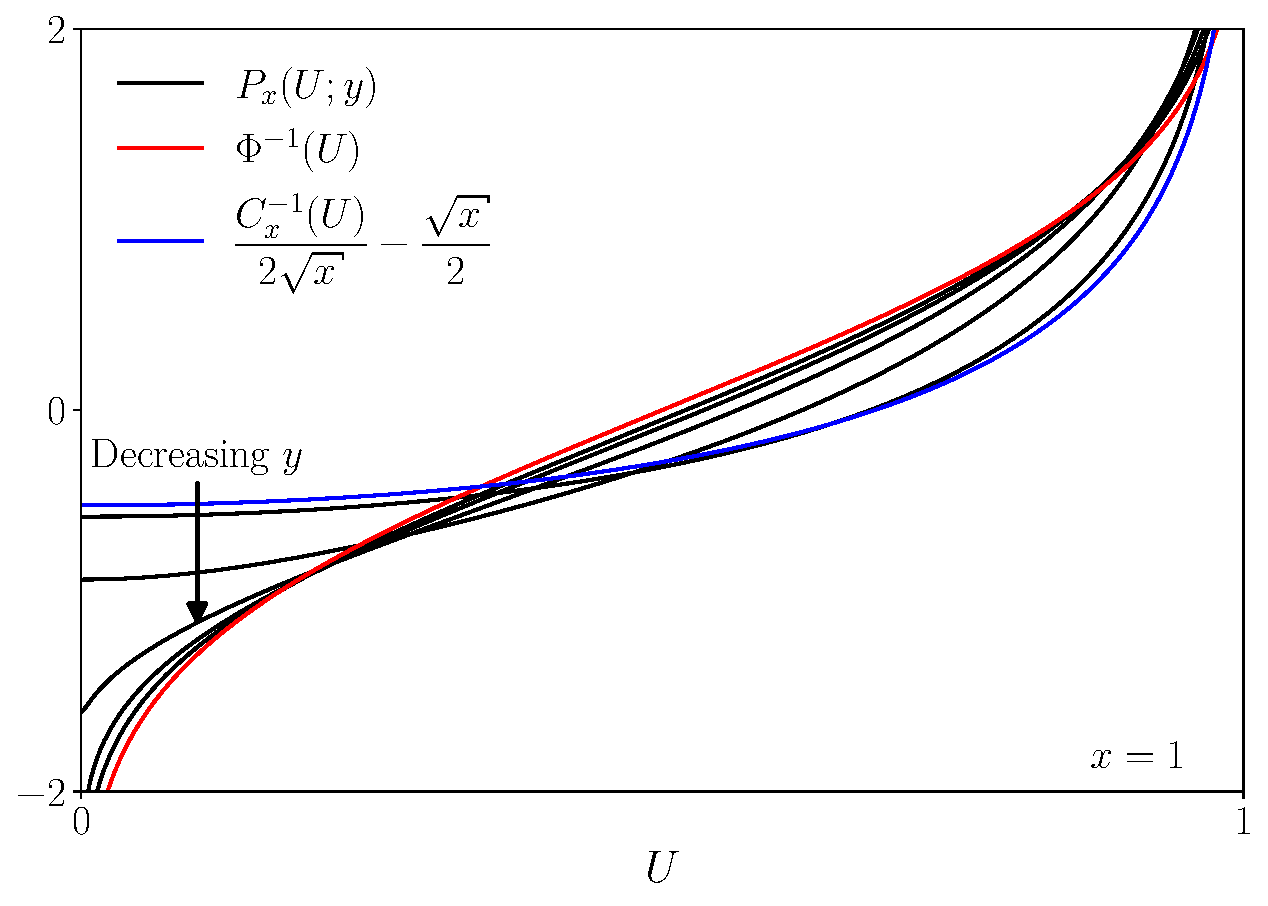
\includegraphics[width=0.7\linewidth]{cir_update_factor_convergence_to_gaussian_both_limits}
\caption{The limiting convergence of the non-central $ \chi^2 $-distribution.}
\label{fig:cir_update_factor_convergence_to_gaussian_both_limits}
\end{figure}

We notice that $ P_x(\cdot;y) $ is not symmetric, but given it looks so similar to the Gaussian, we approximate it similarly. We again use a piecewise polynomial approximation using dyadic intervals. However, as it is not rotationally symmetric, we use one approximation between 0 and $ \tfrac{1}{2} $, and a second between $ \tfrac{1}{2} $ and 1. 

As we have a parametrised distribution for $ 0 < y < 1 $, we construct several approximations for a discrete set of different and equally spaced values of $ \sqrt{y} $, where the value for some specific $ y $ is obtained from linear interpolation in the value of $ \sqrt{y} $. 

A polynomial approximation to the non-central $ \chi^2 $-distribution's inverse cumulative distribution function, produced in the way we've highlighted, is implemented in \singlecodeline{approximate_non_central_chi_squared.py}
and its use is demonstrated in the file \singlecodeline{approximate_non_central_chi_squared_demonstrations.py} with the function \singlecodeline{plot_non_central_chi_squared_polynomial_approximation}
which produces the approximations shown in \Cref{fig:piecewise_polynomial_approximation_of_non_central_chi_squared}.

\begin{figure}[htb]
\centering
\includegraphics[width=0.7\linewidth]{piecewise_polynomial_approximation_of_non_central_chi_squared}
\caption{Several piecewise polynomial approximations using dyadic intervals.}
\label{fig:piecewise_polynomial_approximation_of_non_central_chi_squared}
\end{figure}

Similar to before, we can compare the relative time taken between the exact function and our polynomial approximation using the function \singlecodeline{non_central_chi_squared_polynomial_approximation_timing}
which outputs
\begin{verbatim}
nu       1    5    10   50
lambda                    
1       1.3  1.5  1.5  2.0
5       1.5  1.7  1.7  2.2
10      2.0  2.1  2.4  2.7
50      3.7  3.9  3.9  5.2
\end{verbatim}
and a more comprehensive collection of results are presented in \Cref{tab:non_central_chi_2_times_python_approximation}. We can see from this that our Python implementation is usually slightly faster than the exact function when $ \nu $ and $ \lambda $ are both $ \order{1} $. However, as $ \lambda $ increases such that $ \lambda \gg 1 $ we can see that even our modest Python implementation is much faster. 

\begin{table}[htb]
\centering    
\begin{tabular}{|r|rrrrr|}
\multicolumn{1}{c}{\multirow{2}{*}{$ \lambda $}} & \multicolumn{5}{c}{$ \nu $} \\
\cline{2-6}
\multicolumn{1}{c|}{} & 1 &   5  &  10 &  50  & 100 \\
\hline
   1 &  1.2 &  1.5 &  1.5 &  2.1 &  2.7 \\
   5 &  1.2 &  1.7 &  1.8 &  2.3 &  3.2 \\
  10 &  1.2 &  2.2 &  2.3 &  2.6 &  3.7 \\
  50 &  4.0 &  3.9 &  3.8 &  5.4 &  5.4 \\
 100 &  6.7 &  7.3 &  7.4 &  7.2 &  6.8 \\
 200 &  8.9 &  9.3 &  8.8 &  8.7 &  8.0 \\
 500 & 16.8 & 16.8 & 16.3 & 16.5 & 16.0 \\
1000 & 17.4 & 17.4 & 15.9 & 16.6 & 17.8 \\
\hline 
\end{tabular}\\[1em]
\caption{The relative time required in Python using \texttt{ncx2.ppf} from Scipy's \texttt{scipy.stats} against our polynomial approximation.}
\label{tab:non_central_chi_2_times_python_approximation}
\end{table}


Again, we can implement the same functionality in C, which we can expect to obtain a better performance. The C implementation is found in \singlecodeline{piecewise_linear_approximation_non_central_chi_squared.c} and is depicted in \Cref{code:c:piecewise_linear_approximation_non_central_chi_squared}. A near identical C++ version can also be found in \singlecodeline{piecewise_linear_approximation_non_central_chi_squared.cpp} where the C and C++ codes are built using \singlecodeline{make_time_piecewise_linear_approximation_non_central_chi_squared.sh} and \singlecodeline{make_time_piecewise_linear_approximation_non_central_chi_squared_cpp.sh}
respectively. We can compare these implementations against exact function implementations, such as the CDFLIB library (C and Fortran version are available), and also against the Boost C++ library. The computational savings are shown in \Cref{tab:implementation_times_chi}, from which we can see colossal savings are possible using our approximations. 

\begin{table}[htb]
\hfil 
\subfloat[C implementation (compared against CDFLIB).\label{tab:implementation_times_chi_c}]{
\begin{tabular}{|r|rrrrr|}
\multicolumn{1}{c}{\multirow{2}{*}{$ \lambda $}} & \multicolumn{5}{c}{$ \nu $} \\
\cline{2-6}
\multicolumn{1}{c|}{} & 1 &   5  &  10 &  50  & 100 \\
\hline
1    &    333&   412&   458&   666&   864\\
5    &    391&   447&   534&   701&   966\\
10   &    600&   668&   724&   801&   992\\
50   &   1411&  1424&  1231&  1811&  1811\\
100  &   2271&  2174&  2164&  2207&  2029\\
200  &   2539&  2624&  2791&  2304&  2113\\
500  &   5020&  4912&  4860&  4908&  4886\\
1000 &   4822&  4859&  4866&  4791&  4980\\
\hline
\end{tabular}
}\hfil
\subfloat[C++ implementation (compared against Boost).\label{tab:implementation_times_chi_cpp}]{
\begin{tabular}{|r|rrrrr|}
\multicolumn{1}{c}{\multirow{2}{*}{$ \lambda $}} & \multicolumn{5}{c}{$ \nu $} \\
\cline{2-6}
\multicolumn{1}{c|}{} & 1 &   5  &  10 &  50  & 100 \\
\hline
1    &    671&  1643&  1534&  1734&  2093\\
5    &   1884&  1831&  1733&  2037&  2344\\
10   &   1924&  1937&  1863&  2490&  2490\\
50   &   2576&  2565&  2876&  2945&  2974\\
100  &   3238&  3265&  3255&  3299&  3354\\
200  &   4382&  4384&  4373&  4356&  4333\\
500  &   5260&  5294&  5243&  5249&  5224\\
1000 &   6101&  6022&  6026&  6147&  6093\\
\hline
\end{tabular}
}\hfil\\[1em] 

\caption{The computing ratio between the exact function and the piecewise linear approximation.}
\label{tab:implementation_times_chi}
\end{table}

\begin{lstfloat}[h!tb]
\begin{lstlisting}[style=C, captionpos=b, caption={Piecewise linear approximation for the non-central $ chi^2 $-distribution.}, label={code:c:piecewise_linear_approximation_non_central_chi_squared}]
#include "piecewise_linear_approximation_non_central_chi_squared.h"
#include "piecewise_linear_approximation_non_central_chi_squared_coefficients.h"

#define DOF 1.0f
#define TABLE_SIZE 16
#define INTERPOLATION_FUNCTIONS 16
#define HALVES 2

#pragma omp declare simd
static inline float32 polynomial_approximation(float32 u, 
    uint32 b, uint32 h, uint32 i) 
{ 
    float32 poly_coef_0 = polynomial_coefficients[h][i][0][b];
    float32 poly_coef_1 = polynomial_coefficients[h][i][1][b];
    return poly_coef_0 + poly_coef_1 * u;
}

#pragma omp declare simd
static inline uint32 get_table_index_from_float_format(float32 u);

#pragma omp declare simd
static inline void interpolation_indices(const float32 y, 
    uint32 * restrict interpolation_index_lower, 
    uint32 * restrict interpolation_index_upper, 
    float32 * restrict weight_lower, float32 * restrict weight_upper)
{
    float32 x = sqrtf(y) * (INTERPOLATION_FUNCTIONS - 1);
    *interpolation_index_lower = (uint32) x;
    *interpolation_index_upper = *interpolation_index_lower + 1;
    *weight_upper = x - ((uint32) x);
    *weight_lower = 1.0f - *weight_upper;
}

void piecewise_polynomial_approximation_non_central_chi_squared(
    unsigned int n_samples, const float32 *restrict input, 
    const float32 *restrict non_centrality, float32 *restrict output)
{
#pragma omp simd
    for (unsigned int i = 0; i < n_samples; i++)
    {
        float32 u, p, z, lambda;
        u = input[i];
        lambda = non_centrality[i];
        uint32 upper_half = u > 0.5f;
        u = upper_half ? 1.0f - u : u;
        float32 weight_lower, weight_upper;
        uint32 interpolation_index_lower, interpolation_index_upper;
        float32 y = DOF / (lambda + DOF); // interpolation_value
        interpolation_indices(y, &interpolation_index_lower,
            &interpolation_index_upper, &weight_lower, &weight_upper);
        uint32 b = get_table_index_from_float_format(u);
        float32 p_lower = polynomial_approximation(u, b, upper_half, 
            interpolation_index_lower);
        float32 p_upper = polynomial_approximation(u, b, upper_half, 
            interpolation_index_upper);
        p = weight_lower * p_lower + weight_upper * p_upper;
        z = lambda + DOF + 2.0f * sqrtf(lambda + DOF) * p;
        output[i] = z;
    }
}
\end{lstlisting}
\end{lstfloat}






\clearpage
\section{Monte Carlo simulations using the Euler-Maruyama scheme}

We mentioned in \Cref{sec:when_would_i_use_approximate_random_variables} that random variables (and hence also approximate random variables) play a central role in Monte Carlo simulations, and we will elaborate a bit more on this here. There are many classical problems which can be described by what's called a \emph{first order ordinary differential equation}, which takes the form 
\begin{align}
\dv{x}{t} & = a(t, x), \\
\shortintertext{and is often written as}
\dd{x} & = a(t, x) \dd{t}. \label{eqt:first_order_ode}
\end{align}
Examples of problems taking the form of \Cref{eqt:first_order_ode} can be found in models for: population growth, thermal cooling, circuit theory, and projectile motion. How these systems evolve is not at all random, but completely deterministic. 

Naturally though, there are systems which are subject to random effects which influence how they evolve. Examples of systems experiencing random influences can be found in models from finance, dilute chemistry, and various branches of physics. If a system behaves randomly we say it is \emph{stochastic}, and these can regularly be described by using what's called a \emph{stochastic differential equation} of the form
\begin{equation}
\dd{X_t}  = a(t, X_t) \dd{t} + b(t, X_t) \dd{W_t}. \label{eqt:sde}
\end{equation}
The new term $ \dd{W_t} $ is the underlying stochastic process, where $ W_t $ is called a \emph{Brownian motion}. The most important thing about a Brownian motion is that between two times $ s $ and $ t $, with $ s < t $, the change $ W_t - W_s $ is a zero mean Gaussian random variable with variance $ t - s $. This means that over a time interval $ \Delta t $, the change in the  Brownian motion $ \Delta W_t $ can be expressed using a standard Gaussian random variable $ Z $ by $ \Delta W_t = \sqrt{\Delta t} Z $.

When simulating a path described by \Cref{eqt:sde}, it is important not to forgetting that no two simulations of \Cref{eqt:sde} will be the same, as each path is subjected to unique random influences, as was demonstrated in \Cref{fig:example_simulation}. 

A popular and robust way to simulate processes described by \Cref{eqt:sde} up to  time $ T $ is to use \emph{the Euler-Maruyama scheme}, which makes the approximation
\begin{equation}
\Delta X_t \approx  a(t, X_t) \Delta t + b(t, X_t) \Delta W_t, \label{eqt:euler_maruyama_approximation}
\end{equation}
which gives rise to the Euler-Maruyama scheme 
\begin{equation}
\hat{X}_{n+1} = \hat{X}_n +  a(t_n, \hat{X}_n) \delta + b(t_n, \hat{X}_n) \sqrt{\delta} Z_n, \label{eqt:euler_maruyama_scheme}
\end{equation}
where we simulate from $ \hat{X}_0 \to \hat{X}_1 \to \hat{X}_2 \to \cdots \to \hat{X}_n \to \cdots \to \hat{X}_N $, using $ N $ equally spaced time increments $ \delta = \tfrac{T}{N}$ where $ t_n = n \delta $. 

To estimate exactly where the final position $ X_T $ is expected to be, the Monte Carlo scheme uses $ M $ simulations to approximate
\begin{equation}
\conExp{X_T} \approx \conExp{\hat{X}_N} \approx \dfrac{1}{M} \sum^M \hat{X}_N.
\end{equation}
Performing all these $ M $ simulations, each requiring $ N $ random numbers, the amount of random numbers used can quickly become enormous, and generating them becomes the computational bottleneck. This is where our approximate random variables come into play. Instead of the random variables $ Z_n $, which exactly follow the Gaussian distribution, we propose using approximate random variables $ \tilde{Z}_n $ and the modified version of the Euler-Maruyama scheme
\begin{equation}
\tilde{X}_{n+1} = \tilde{X}_n +  a(t_n, \tilde{X}_n) \delta + b(t_n, \tilde{X}_n) \sqrt{\delta} \tilde{Z}_n. \label{eqt:euler_maruyama_scheme_approximate_random_variables}
\end{equation}

Switching to the modified Euler-Maruyama scheme will give a considerable speed improvement, but it will introduce some error. Is there a way to benefit from the increased speed but without losing accuracy? Fortunately, there is an extension of regular Monte Carlo called \emph{multilevel Monte Carlo} which does just this, and the idea behind it is surprisingly simple. We suppose that in some setting we have the means to run simulations in some very high fidelity with a high computational cost, or a low fidelity with a low computational cost, where these are approximations to some exact quantity. By convention we denote these as \emph{fine} and \emph{coarse} simulations respectively.  The multilevel estimate uses the combination
\begin{equation}
\rlap{$\overbrace{\phantom{\mathbb{E}(X_{\mathrm{exact}}) \approx \mathbb{E}(X_{\mathrm{fine}})}}^{\mathclap{\text{Regular Monte Carlo}}}$} \mathbb{E}(X_{\mathrm{exact}}) \approx \underbrace{\mathbb{E}(X_{\mathrm{fine}}) = \mathbb{E}(X_{\mathrm{coarse}}) + \mathbb{E}(X_{\mathrm{fine}} - X_{\mathrm{coarse}})}_{\text{Multilevel Monte Carlo}}. \label{eqt:mlmc}
\end{equation}


If we inspect the portion marked regular Monte Carlo, everything is as one might expect, and we would estimate the exact quantity using the finest resolution possible. The interesting bit is the equality we've marked as the multilevel Monte Carlo. The fact that this is an equality means that the same accuracy as the regular Monte Carlo is achieved, and no accuracy is lost. So why change to the multilevel scheme? The multilevel scheme's first expectation $ \mathbb{E}(X_{\mathrm{coarse}}) $ is our new primary estimation tool, which we can see is made from coarse simulations, and so is computationally  cheaper, giving a speed improvement. The second expectation $ \mathbb{E}(X_{\mathrm{fine}} - X_{\mathrm{coarse}}) $ is the correction needed to adjust from a coarse simulation to a fine simulation, and is how the fine simulation's accuracy is maintained. This second expectation only requires a negligible number of simulations, and hence doesn't affect the overall cost. This is why the multilevel scheme has all the speed of a coarse simulation and the accuracy of a fine simulation. Using this multilevel Monte Carlo, the higher fidelity simulations are produced from the Euler-Maruyama scheme using the exact random numbers, and faster but lower fidelity simulations are produced using the approximate random numbers. We gain speed without losing accuracy.

Usually the fine and coarse simulations differ by using smaller and larger time increments. Our approximate random variables present a separate way to boost speed without losing performance. Unfortunately, incorporating approximate random variables into a pre-existing regular Monte Carlo or multilevel Monte Carlo is not without some technical difficulties. Approximate random variables cannot be used for all simulations, there are limitations, and these are too mathematically technical to repeat here. For anyone looking to implement a  Monte Carlo scheme using them, we recommend reading some of the more advanced material mentioned in \Cref{sec:where_can_i_learn_more}.



\end{document}
